        %%******************************************%%
        %%                                          %%
        %%        Modello di tesi di laurea         %%
        %%            di Andrea Giraldin            %%
        %%                                          %%
        %%             2 novembre 2012              %%
        %%                                          %%
        %%******************************************%%


% I seguenti commenti speciali impostano:
% 1. 
% 2. PDFLaTeX come motore di composizione;
% 3. tesi.tex come documento principale;
% 4. il controllo ortografico italiano per l'editor.

% !TEX encoding = UTF-8
% !TEX TS-program = pdflatex
% !TEX root = tesi.tex
% !TEX spellcheck = it-IT

% PDF/A filecontents
\RequirePackage{filecontents}
\begin{filecontents*}{\jobname.xmpdata}
  \Title{Document’s title}
  \Author{Author’s name}
  \Language{it-IT}
  \Subject{The abstract, or short description.}
  \Keywords{keyword1\sep keyword2\sep keyword3}
\end{filecontents*}

\documentclass[10pt,                    % corpo del font principale
               a4paper,                 % carta A4
               twoside,                 % impagina per fronte-retro
               openright,               % inizio capitoli a destra
               english,                 
               italian,                 
               ]{book}    

%**************************************************************
% Importazione package
%************************************************************** 

\PassOptionsToPackage{dvipsnames}{xcolor} % colori PDF/A

\usepackage{colorprofiles}

\usepackage[a-2b,mathxmp]{pdfx}[2018/12/22]
                                        % configurazione PDF/A
                                        % validare in https://www.pdf-online.com/osa/validate.aspx

%\usepackage{amsmath,amssymb,amsthm}    % matematica

\usepackage[T1]{fontenc}                % codifica dei font:
                                        % NOTA BENE! richiede una distribuzione *completa* di LaTeX

\usepackage[utf8]{inputenc}             % codifica di input; anche [latin1] va bene
                                        % NOTA BENE! va accordata con le preferenze dell'editor

\usepackage[english, italian]{babel}    % per scrivere in italiano e in inglese;
                                        % l'ultima lingua (l'italiano) risulta predefinita

\usepackage{bookmark}                   % segnalibri

\usepackage{caption}                    % didascalie

\usepackage{chngpage,calc}              % centra il frontespizio

\usepackage{csquotes}                   % gestisce automaticamente i caratteri (")

\usepackage{emptypage}                  % pagine vuote senza testatina e piede di pagina

\usepackage{epigraph}			% per epigrafi

\usepackage{eurosym}                    % simbolo dell'euro

%\usepackage{indentfirst}               % rientra il primo paragrafo di ogni sezione

\usepackage{graphicx}                   % immagini

\usepackage{hyperref}                   % collegamenti ipertestuali

\usepackage[binding=5mm]{layaureo}      % margini ottimizzati per l'A4; rilegatura di 5 mm

\usepackage{listings}                   % codici

\usepackage{microtype}                  % microtipografia

\usepackage{mparhack,fixltx2e,relsize}  % finezze tipografiche

\usepackage{nameref}                    % visualizza nome dei riferimenti                                      
\usepackage[font=small]{quoting}        % citazioni

\usepackage{subfig}                     % sottofigure, sottotabelle

\usepackage[italian]{varioref}          % riferimenti completi della pagina

\usepackage{booktabs}                   % tabelle                                       
\usepackage{tabularx}                   % tabelle di larghezza prefissata                                    
\usepackage{longtable}                  % tabelle su più pagine                                        
\usepackage{ltxtable}                   % tabelle su più pagine e adattabili in larghezza

\usepackage[toc, acronym]{glossaries}   % glossario
                                        % per includerlo nel documento bisogna:
                                        % 1. compilare una prima volta tesi.tex;
                                        % 2. eseguire: makeindex -s tesi.ist -t tesi.glg -o tesi.gls tesi.glo
                                        % 3. eseguire: makeindex -s tesi.ist -t tesi.alg -o tesi.acr tesi.acn
                                        % 4. compilare due volte tesi.tex.

\usepackage[backend=biber,style=verbose-ibid,hyperref,backref]{biblatex}
                                        % eccellente pacchetto per la bibliografia; 
                                        % produce uno stile di citazione autore-anno; 
                                        % lo stile "numeric-comp" produce riferimenti numerici
                                        % per includerlo nel documento bisogna:
                                        % 1. compilare una prima volta tesi.tex;
                                        % 2. eseguire: biber tesi
                                        % 3. compilare ancora tesi.tex.

\usepackage{float}

%**************************************************************
% file contenente le impostazioni della tesi
%**************************************************************

%**************************************************************
% Frontespizio
%**************************************************************

% Autore
\newcommand{\myName}{Gabriel Bizzo}                                    
\newcommand{\myTitle}{Confronto tra Angular e React nella realizzazione di una piattaforma di e-Voting}

% Tipo di tesi                   
\newcommand{\myDegree}{Tesi di laurea triennale}

% Università             
\newcommand{\myUni}{Università degli Studi di Padova}

% Facoltà       
\newcommand{\myFaculty}{Corso di Laurea in Informatica}

% Dipartimento
\newcommand{\myDepartment}{Dipartimento di Matematica "Tullio Levi-Civita"}

% Titolo del relatore
\newcommand{\profTitle}{Prof.}

% Relatore
\newcommand{\myProf}{Gilberto Filè}

% Luogo
\newcommand{\myLocation}{Padova}

% Anno accademico
\newcommand{\myAA}{2020-2021}

% Data discussione
\newcommand{\myTime}{Settembre 2021}


%**************************************************************
% Impostazioni di impaginazione
% see: http://wwwcdf.pd.infn.it/AppuntiLinux/a2547.htm
%**************************************************************

\setlength{\parindent}{14pt}   % larghezza rientro della prima riga
\setlength{\parskip}{0pt}   % distanza tra i paragrafi


%**************************************************************
% Impostazioni di biblatex
%**************************************************************
\bibliography{bibliografia} % database di biblatex 

\defbibheading{bibliography} {
    \cleardoublepage
    \phantomsection 
    \addcontentsline{toc}{chapter}{\bibname}
    \chapter*{\bibname\markboth{\bibname}{\bibname}}
}

\setlength\bibitemsep{1.5\itemsep} % spazio tra entry

\DeclareBibliographyCategory{opere}
\DeclareBibliographyCategory{web}

\addtocategory{opere}{womak:lean-thinking}
\addtocategory{web}{site:agile-manifesto}

\defbibheading{opere}{\section*{Riferimenti bibliografici}}
\defbibheading{web}{\section*{Siti Web consultati}}


%**************************************************************
% Impostazioni di caption
%**************************************************************
\captionsetup{
    tableposition=top,
    figureposition=bottom,
    font=small,
    format=hang,
    labelfont=bf
}

%**************************************************************
% Impostazioni di glossaries
%**************************************************************

%**************************************************************
% Acronimi
%**************************************************************
\renewcommand{\acronymname}{Acronimi e abbreviazioni}

\newacronym[description={\glslink{apig}{Application Program Interface}}]
    {api}{API}{Application Program Interface}

\newacronym[description={\glslink{umlg}{Unified Modeling Language}}]
    {uml}{UML}{Unified Modeling Language}

%**************************************************************
% Glossario
%**************************************************************
%\renewcommand{\glossaryname}{Glossario}

\newglossaryentry{apig}
{
    name=\glslink{api}{API},
    text=Application Program Interface,
    sort=api,
    description={in informatica con il termine \emph{Application Programming Interface API} (ing. interfaccia di programmazione di un'applicazione) si indica ogni insieme di procedure disponibili al programmatore, di solito raggruppate a formare un set di strumenti specifici per l'espletamento di un determinato compito all'interno di un certo programma. La finalità è ottenere un'astrazione, di solito tra l'hardware e il programmatore o tra software a basso e quello ad alto livello semplificando così il lavoro di programmazione}
}

\newglossaryentry{umlg}
{
    name=\glslink{uml}{UML},
    text=UML,
    sort=uml,
    description={in ingegneria del software \emph{UML, Unified Modeling Language} (ing. linguaggio di modellazione unificato) è un linguaggio di modellazione e specifica basato sul paradigma object-oriented. L'\emph{UML} svolge un'importantissima funzione di ``lingua franca'' nella comunità della progettazione e programmazione a oggetti. Gran parte della letteratura di settore usa tale linguaggio per descrivere soluzioni analitiche e progettuali in modo sintetico e comprensibile a un vasto pubblico}
}
 % database di termini
\makeglossaries


%**************************************************************
% Impostazioni di graphicx
%**************************************************************
\graphicspath{{immagini/}} % cartella dove sono riposte le immagini


%**************************************************************
% Impostazioni di hyperref
%**************************************************************
\hypersetup{
    %hyperfootnotes=false,
    %pdfpagelabels,
    %draft,	% = elimina tutti i link (utile per stampe in bianco e nero)
    colorlinks=true,
    linktocpage=true,
    pdfstartpage=1,
    pdfstartview=,
    % decommenta la riga seguente per avere link in nero (per esempio per la stampa in bianco e nero)
    %colorlinks=false, linktocpage=false, pdfborder={0 0 0}, pdfstartpage=1, pdfstartview=FitV,
    breaklinks=true,
    pdfpagemode=UseNone,
    pageanchor=true,
    pdfpagemode=UseOutlines,
    plainpages=false,
    bookmarksnumbered,
    bookmarksopen=true,
    bookmarksopenlevel=1,
    hypertexnames=true,
    pdfhighlight=/O,
    %nesting=true,
    %frenchlinks,
    urlcolor=webbrown,
    linkcolor=RoyalBlue,
    citecolor=webgreen,
    %pagecolor=RoyalBlue,
    %urlcolor=Black, linkcolor=Black, citecolor=Black, %pagecolor=Black,
    pdftitle={\myTitle},
    pdfauthor={\textcopyright\ \myName, \myUni, \myFaculty},
    pdfsubject={},
    pdfkeywords={},
    pdfcreator={pdfLaTeX},
    pdfproducer={LaTeX}
}

%**************************************************************
% Impostazioni di itemize
%**************************************************************
\renewcommand{\labelitemi}{$\ast$}

%\renewcommand{\labelitemi}{$\bullet$}
%\renewcommand{\labelitemii}{$\cdot$}
%\renewcommand{\labelitemiii}{$\diamond$}
%\renewcommand{\labelitemiv}{$\ast$}


%**************************************************************
% Impostazioni di listings
%**************************************************************
\lstset{
    language=[LaTeX]Tex,%C++,
    keywordstyle=\color{RoyalBlue}, %\bfseries,
    basicstyle=\small\ttfamily,
    %identifierstyle=\color{NavyBlue},
    commentstyle=\color{Green}\ttfamily,
    stringstyle=\rmfamily,
    numbers=none, %left,%
    numberstyle=\scriptsize, %\tiny
    stepnumber=5,
    numbersep=8pt,
    showstringspaces=false,
    breaklines=true,
    frameround=ftff,
    frame=single
} 


%**************************************************************
% Impostazioni di xcolor
%**************************************************************
\definecolor{webgreen}{rgb}{0,.5,0}
\definecolor{webbrown}{rgb}{.6,0,0}


%**************************************************************
% Altro
%**************************************************************

\newcommand{\omissis}{[\dots\negthinspace]} % produce [...]

% eccezioni all'algoritmo di sillabazione
\hyphenation
{
    ma-cro-istru-zio-ne
    gi-ral-din
}

\newcommand{\sectionname}{sezione}
\addto\captionsitalian{\renewcommand{\figurename}{Figura}
                       \renewcommand{\tablename}{Tabella}}

\newcommand{\glsfirstoccur}{\ap{{[g]}}}

\newcommand{\intro}[1]{\emph{\textsf{#1}}}

%**************************************************************
% Environment per ``rischi''
%**************************************************************
\newcounter{riskcounter}                % define a counter
\setcounter{riskcounter}{0}             % set the counter to some initial value

%%%% Parameters
% #1: Title
\newenvironment{risk}[1]{
    \refstepcounter{riskcounter}        % increment counter
    \par \noindent                      % start new paragraph
    \textbf{\arabic{riskcounter}. #1}   % display the title before the 
                                        % content of the environment is displayed 
}{
    \par\medskip
}

\newcommand{\riskname}{Rischio}

\newcommand{\riskdescription}[1]{\textbf{\\Descrizione:} #1.}

\newcommand{\risksolution}[1]{\textbf{\\Soluzione:} #1.}

%**************************************************************
% Environment per ``use case''
%**************************************************************
\newcounter{usecasecounter}             % define a counter
\setcounter{usecasecounter}{0}          % set the counter to some initial value

%%%% Parameters
% #1: ID
% #2: Nome
\newenvironment{usecase}[2]{
    \renewcommand{\theusecasecounter}{\usecasename #1}  % this is where the display of 
                                                        % the counter is overwritten/modified
    \refstepcounter{usecasecounter}             % increment counter
    \vspace{10pt}
    \par \noindent                              % start new paragraph
    {\large \textbf{\usecasename #1: #2}}       % display the title before the 
                                                % content of the environment is displayed 
    \medskip
}{
    \medskip
}

\newcommand{\usecasename}{UC}

\newcommand{\usecaseactors}[1]{\textbf{\\Attori Principali:} #1. \vspace{4pt}}
\newcommand{\usecasepre}[1]{\textbf{\\Precondizioni:} #1. \vspace{4pt}}
\newcommand{\usecasedesc}[1]{\textbf{\\Descrizione:} #1. \vspace{4pt}}
\newcommand{\usecasepost}[1]{\textbf{\\Postcondizioni:} #1. \vspace{4pt}}
\newcommand{\usecasealt}[1]{\textbf{\\Scenario Alternativo:} #1. \vspace{4pt}}

%**************************************************************
% Environment per ``namespace description''
%**************************************************************

\newenvironment{namespacedesc}{
    \vspace{10pt}
    \par \noindent                              % start new paragraph
    \begin{description} 
}{
    \end{description}
    \medskip
}

\newcommand{\classdesc}[2]{\item[\textbf{#1:}] #2}
                     % file con le impostazioni personali

\begin{document}
%**************************************************************
% Materiale iniziale
%**************************************************************
\frontmatter
% !TEX encoding = UTF-8
% !TEX TS-program = pdflatex
% !TEX root = ../tesi.tex

%**************************************************************
% Frontespizio 
%**************************************************************
\begin{titlepage}

\begin{center}

\begin{LARGE}
\textbf{\myUni}\\
\end{LARGE}

\vspace{10pt}

\begin{Large}
\textsc{\myDepartment}\\
\end{Large}

\vspace{10pt}

\begin{large}
\textsc{\myFaculty}\\
\end{large}

\vspace{30pt}
\begin{figure}[htbp]
\begin{center}

\includegraphics[height=6cm]{logo-unipd}
\end{center}
\end{figure}
\vspace{30pt} 

\begin{LARGE}
\begin{center}
\textbf{\myTitle}\\
\end{center}
\end{LARGE}

\vspace{10pt} 

\begin{large}
\textsl{\myDegree}\\
\end{large}

\vspace{40pt} 

\begin{large}
\begin{flushleft}
\textit{Relatore}\\ 
\vspace{5pt} 
\profTitle \myProf
\end{flushleft}

\vspace{0pt} 

\begin{flushright}
\textit{Laureando}\\ 
\vspace{5pt} 
\myName
\end{flushright}
\end{large}

\vspace{40pt}

\line(1, 0){338} \\
\begin{normalsize}
\textsc{Anno Accademico \myAA}
\end{normalsize}

\end{center}
\end{titlepage} 
% !TEX encoding = UTF-8
% !TEX TS-program = pdflatex
% !TEX root = ../tesi.tex

%**************************************************************
% Colophon
%**************************************************************
\clearpage
\phantomsection
\thispagestyle{empty}

\hfill

\vfill

\noindent\myName: \textit{\myTitle,}
\myDegree,
\textcopyright\ \myTime.
% !TEX encoding = UTF-8
% !TEX TS-program = pdflatex
% !TEX root = ../tesi.tex

%**************************************************************
% Sommario
%**************************************************************
\cleardoublepage
\phantomsection
\pdfbookmark{Sommario}{Sommario}
\begingroup
\let\clearpage\relax
\let\cleardoublepage\relax
\let\cleardoublepage\relax

\chapter*{Sommario}

Il presente documento descrive il lavoro svolto durante il periodo di stage, della durata di circa trecento ore, dal laureando Gabriel Bizzo presso l'azienda Sync Lab S.r.l.
Gli obbiettivi da raggiungere erano molteplici.\\

In primo luogo era richiesto lo sviluppo di ...
In secondo luogo era richiesta l'implementazione di un ... 

Terzo ed ultimo obbiettivo era l'integrazione ...

%\vfill
%
%\selectlanguage{english}
%\pdfbookmark{Abstract}{Abstract}
%\chapter*{Abstract}
%
%\selectlanguage{italian}

\endgroup			

\vfill


% !TEX encoding = UTF-8
% !TEX TS-program = pdflatex
% !TEX root = ../tesi.tex

%**************************************************************
% Ringraziamenti
%**************************************************************
\cleardoublepage
\phantomsection
\pdfbookmark{Ringraziamenti}{ringraziamenti}

\begin{flushright}{
	\slshape    
	``Life is really simple, but we insist on making it complicated''} \\ 
	\medskip
    --- Confucius
\end{flushright}


\bigskip

\begingroup
\let\clearpage\relax
\let\cleardoublepage\relax
\let\cleardoublepage\relax

\chapter*{Ringraziamenti}

\noindent \textit{Innanzitutto, vorrei esprimere la mia gratitudine al Prof. NomeDelProfessore, relatore della mia tesi, per l'aiuto e il sostegno fornitomi durante la stesura del lavoro.}\\

\noindent \textit{Desidero ringraziare con affetto i miei genitori per il sostegno, il grande aiuto e per essermi stati vicini in ogni momento durante gli anni di studio.}\\

\noindent \textit{Ho desiderio di ringraziare poi i miei amici per tutti i bellissimi anni passati insieme e le mille avventure vissute.}\\
\bigskip

\noindent\textit{\myLocation, \myTime}
\hfill \myName

\endgroup


% !TEX encoding = UTF-8
% !TEX TS-program = pdflatex
% !TEX root = ../tesi.tex

%**************************************************************
% Indici
%**************************************************************
\cleardoublepage
\pdfbookmark{\contentsname}{tableofcontents}
\setcounter{tocdepth}{2}
\tableofcontents
%\markboth{\contentsname}{\contentsname} 
\clearpage

\begingroup 
    \let\clearpage\relax
    \let\cleardoublepage\relax
    \let\cleardoublepage\relax
    %*******************************************************
    % Elenco delle figure
    %*******************************************************    
    \phantomsection
    \pdfbookmark{\listfigurename}{lof}
    \listoffigures

    \vspace*{8ex}

    %*******************************************************
    % Elenco delle tabelle
    %*******************************************************
    \phantomsection
    \pdfbookmark{\listtablename}{lot}
    \listoftables
        
    \vspace*{8ex}
\endgroup

\cleardoublepage

\cleardoublepage

%**************************************************************
% Materiale principale
%**************************************************************
\mainmatter
% !TEX encoding = UTF-8
% !TEX TS-program = pdflatex
% !TEX root = ../tesi.tex

%**************************************************************
\chapter{Introduzione}
\label{cap:introduzione}
%**************************************************************

% ESEMPI

%\noindent Esempio di utilizzo di un termine nel glossario \\
%\gls{api}. \\

%\noindent Esempio di citazione in linea \\
%\cite{site:agile-manifesto}. \\

%\noindent Esempio di citazione nel pie' di pagina \\
%citazione\footcite{womak:lean-thinking} \\

%**************************************************************
\section{L'azienda}

Sync Lab nasce come Software house tramutatasi rapidamente in System Integrator attraverso un processo di maturazione delle competenze tecnologiche, metodologiche ed applicative nel dominio del software. \\
L'azienda, propone sul mercato interessanti quanto innovativi prodotti software, nati nel loro laboratorio di ricerca e sviluppo. Attraverso questi prodotti Sync Lab ha gradualmente conquistato significativamente fette di mercato nei seguenti settori: mobile, videosorveglianza e sicurezza delle infrastrutture informatiche aziendali. \\
Attualmente, Sync Lab ha più di 150 clienti diretti e finali, con un organico aziendale di 200 dipendenti distribuiti tra le 5 sedi dislocate in tutta Italia.

\begin{figure}[!h] 
    \centering 
    
\includegraphics[width=0.7\columnwidth]{sync_lab_logo} 
    \caption{Logo dell'azienda Sync Lab}
\end{figure}

%**************************************************************
\section{Scelta dell'azienda}

Il primo contatto avuto con l'azienda Sync Lab è avvenuto allo StageIT 2021, effettuato in modalità telematica. Il presentatore dell'azienda è stato l’ingegnere Fabio Pallaro, il quale ha spiegato in modo chiaro ed esaustivo le caratteristiche dell'azienda. La motivazione principale che mi ha spinto a scegliere Sync Lab è stata la conferma da parte del sig. Pallaro di accontentare gli stagisti rispetto alle loro preferenze nell'ambito informatico, permettendomi di effettuare un approfondimento a tutto tondo nell'ambito dello sviluppo di applicazioni web.

%**************************************************************
\section{Il progetto Voting-Online}

La votazione elettronica, anche detta e-Voting (dall'inglese <<electronic voting>>), consiste in un insieme di metodologie che permettono ai cittadini l'espressione del proprio voto e la gestione delle preferenze attraverso tecnologie elettroniche e informatiche. \\
Gli applicativi software che realizzano questa tipologia di sistema permettono all'utente di accedere ad una maschera per effettuare una votazione, passando precedentemente per una procedura di autenticazione in modo da collegare il voto ad una persona fisica in modo sicuro. Questi sistemi, oltre ad acquisire le preferenze degli elettori, offrono ad un insieme di amministratori della piattaforma degli strumenti per creare e configurare diverse tipologie di elezioni, oltre che per gestire l'inserimento e/o la rimozione dei partiti partecipanti. \\
Il progetto di stage \textit{Voting-Online}, proposto da Sync Lab, consiste nell'analisi, progettazione e realizzazione di un’applicazione web riguardante il suddetto ambito. Tale progetto nasce per mostrare, principalmente ad aziende private, quella che potrebbe essere un'applicazione web di e-Voting attraverso un prototipo. \\
Il progetto in questione si focalizza sullo sviluppo del \gls{frontend}, e quindi sull'approfondimento delle tecnologie ad esso connesse come Angular e React, anche se una parte del lavoro prevede lo studio di Java e del \gls{frameworkg} Spring in modo da acquisire una conoscenza di base anche sul lato \gls{backend}.
L'argomento principale di tale progetto risulta quindi lo sviluppo delle interfacce grafiche corrispondenti alle maschere per fornire le funzionalità necessarie agli utenti e agli amministratori, utilizzando i linguaggi Javascript e Typescript. \\
Lo sviluppo del \gls{frontend}, utilizzando le due tecnologie precedentemente citate, ha permesso di effettuare in conclusione un'attenta analisi comparativa tra di esse, approfondita nell'{\hyperref[cap:angular-react]{apposita sezione}}.

%**************************************************************
\section{Strumenti di sviluppo e di supporto}
\label{sez:strumenti-smartworking}
Strumenti software utilizzati per lo sviluppo, il versionamento e la documentazione dell'applicativo durante le diverse fasi del suo ciclo di vita.

\subsection*{Draw.io}
\textit{Draw.io} è una piattaforma online gratuita per la creazione di varie tipologie di diagrammi, esportabili come file in diversi formati (tra i quali PDF o JPEG). Tra le diverse possibilità offerte  dal software sono presenti i diagrammi di flusso, di processo, \gls{umlg}, \gls{Entita'-Relazione} e di rete. Questa piattaforma è stata utilizzata per creare i diagrammi dei casi d'uso, utilizzati per l'analisi dei requisiti illustrata nel terzo capitolo.

\subsection*{Visual Studio Code}
\textit{Visual Studio Code} è un <<Integrated development environment>> (IDE), ovvero una piattaforma che consente di migliorare l'esperienza di sviluppo software e, tra i vari strumenti che rende disponibile, contiene un editor di codice sorgente. Grazie alle numerose estensioni che è possibile installare, si può utilizzare una vasta gamma di linguaggi di programmazione e funzionalità di supporto alla scrittura del codice. Uno strumento disponibile grazie a questo IDE che risulta molto utile è l'intelliSense, ovvero una forma di completamento automatico del codice e di visualizzazione grafica di informazioni durante lo sviluppo.

\subsection*{Overleaf}
\textit{Overleaf} è un editor LaTeX collaborativo basato su cloud e viene utilizzato per scrivere, modificare e pubblicare varie tipologie di documenti. Questo software è stato utilizzato per la scrittura del documento tecnico, richiesto dall'azienda insieme al codice sorgente.

\subsection*{Git}
\textit{Git} è uno strumento per il controllo di versione distribuito utilizzabile da interfaccia a riga di comando. E' possibile utilizzare il software in questione per collaborare con più membri di un team e per controllare la versione del codice prodotto così da poter ritornare ad una versione stabile in caso di problemi.

%**************************************************************
\section{Strumenti organizzativi}
\label{sez:strumenti-organizzativi}
Strumenti software utilizzati per il coordinamento e la pianificazione in accordo con l'azienda.

\subsection*{Discord}
\textit{Discord} è una piattaforma di VoIP, messaggistica istantanea e distribuzione digitale progettata per la comunicazione tra comunità di videogiocatori, ma utilizzabile per diversi scopi. Gli utenti possono comunicare con chiamate vocali, video-chiamate, messaggi di testo, media e file in chat private o come membri di un server. Questo strumento permette lo scambio di messaggi e materiale digitale tra gli stagisti e i dipendenti dell'azienda in modo facile e veloce.

\subsection*{Google Sheets}
\textit{Google Sheets} è un programma per fogli di calcolo incluso come parte della suite di editor di documenti basata sul Web gratuita offerta da Google. La piattaforma consente agli utenti di creare e modificare file collaborando con altri utenti in tempo reale. Attraverso questo software è stato possibile compilare un diario digitale che ha permesso al tutor aziendale di controllare lo stato di avanzamento del lavoro dello stage in modo accurato e giornaliero.
\subsection*{Notion}
\textit{Notion} è una piattaforma che fornisce componenti come note, database, calendari, promemoria. Gli utenti possono collegare questi componenti per creare i propri sistemi per la gestione della conoscenza, prendere appunti, gestire dati e progetti. L'azienda Sync Lab, sfruttando questo applicativo, gestisce in modo semplice ed efficace la problematica del flusso di persone in ufficio in tempo di pandemia da Covid-19, permettendo di segnalare la propria presenza in sede fino ad un numero massimo di persone raggiungibile ogni giorno.

%**************************************************************
\section{Organizzazione del testo}

\subsection{Struttura del documento}
Il documento, suddiviso in sei capitoli, è strutturato nella seguente modalità:
\begin{description}
    \item[{\hyperref[cap:introduzione]{Il primo capitolo}}] effettua una breve introduzione all'azienda e al lavoro effettuato durante lo stage curricolare presso Sync Lab.

    \item[{\hyperref[cap:descrizione-stage]{Il secondo capitolo}}] descrive lo stage elencando gli obiettivi da raggiungere, la pianificazione del lavoro e l'analisi preventiva dei rischi.
    
    \item[{\hyperref[cap:analisi-requisiti]{Il terzo capitolo}}] approfondisce l'analisi dei requisiti effettuata per il progetto Voting-Online.
    
    \item[{\hyperref[cap:progettazione-codifica]{Il quarto capitolo}}] approfondisce le tecnologie utilizzate nel progetto Voting-Online, la progettazione del \gls{backend} e del \gls{frontend} e una descrizione dettagliata dei relativi software ottenuti dalla loro codifica.
    
    \item[{\hyperref[cap:angular-react]{Il quinto capitolo}}] approfondisce le tecnologie utilizzate per lo sviluppo del \gls{frontend}, ovvero Angular e React, effettuando un confronto tra diversi dettagli tecnici e considerazioni sulle performance.
    
    \item[{\hyperref[cap:conclusioni]{Il sesto capitolo}}] contiene un'analisi del lavoro svolto e le conclusioni tratte.
    
    %\item[{\hyperref[cap:conclusioni]{Nel settimo capitolo}}] descrive ...
\end{description}

\subsection{Convenzioni tipografiche}
Riguardo la stesura del testo, relativamente al documento sono state adottate le seguenti convenzioni tipografiche:
\begin{itemize}
	\item gli acronimi, le abbreviazioni e i termini ambigui o di uso non comune menzionati vengono definiti nel glossario, situato alla fine del presente documento;
	\item per la prima occorrenza dei termini riportati nel glossario viene utilizzata la nomenclatura "\emph{parola(abbreviazione)}", mentre per ogni successiva occorrenza verrà utilizzata solamente l'abbreviazione di tale termine;
	\item i termini in lingua straniera o facenti parti del gergo tecnico sono evidenziati con il carattere \emph{corsivo}.
\end{itemize}             % Introduzione
%% !TEX encoding = UTF-8
% !TEX TS-program = pdflatex
% !TEX root = ../tesi.tex

%**************************************************************
\chapter{Processi e metodologie}
\label{cap:processi-metodologie}
%**************************************************************

\intro{Brevissima introduzione al capitolo}\\

%**************************************************************
\section{Processo sviluppo prodotto}             % Processi e metodologie
% !TEX encoding = UTF-8
% !TEX TS-program = pdflatex
% !TEX root = ../tesi.tex

%**************************************************************
\chapter{Processi e metodologie}
\label{cap:processi-metodologie}
%**************************************************************

\intro{Brevissima introduzione al capitolo}\\

%**************************************************************
\section{Processo sviluppo prodotto}             % Descrizione stage
% !TEX encoding = UTF-8
% !TEX TS-program = pdflatex
% !TEX root = ../tesi.tex

%**************************************************************
\chapter{Analisi dei requisiti}
\label{cap:analisi-requisiti}
%**************************************************************

\intro{In questo capitolo vengono descritte le funzionalità che il prodotto deve offrire elencando i casi d’uso e i requisiti individuati.}\\

\section{Casi d'uso}

Per lo studio dei casi di utilizzo del prodotto sono stati creati dei diagrammi.
I diagrammi dei casi d'uso\footcite{site:UseCase} (\textbf{UC}) sono diagrammi di tipo \gls{umlg} dedicati alla descrizione delle funzioni o servizi offerti da un sistema, così come sono percepiti e utilizzati dagli attori che interagiscono col sistema stesso.

\subsection{Attori principali}
Gli attori principali individuati sono i seguenti:
\begin{itemize}
    \item \textbf{Utente non autenticato}: indica l'utente che non ha effettuato l'autenticazione attraverso la procedura di login. Questo attore non deve avere la possibilità di accedere agli strumenti di voto e a quelli di monitoraggio della piattaforma;
    \item \textbf{Elettore}: indica l'utente che ha effettuato l'accesso alla piattaforma con un profilo da elettore e deve poter accedere agli strumenti di voto;
    \item \textbf{Amministratore}: indica l'utente che ha effettuato l'accesso alla piattaforma con un profilo da amministratore e deve poter accedere agli strumenti di monitoraggio delle votazioni.
\end{itemize}

\subsection{Elenco dei casi d'uso}

\begin{figure}[h!] 
    \centering 
    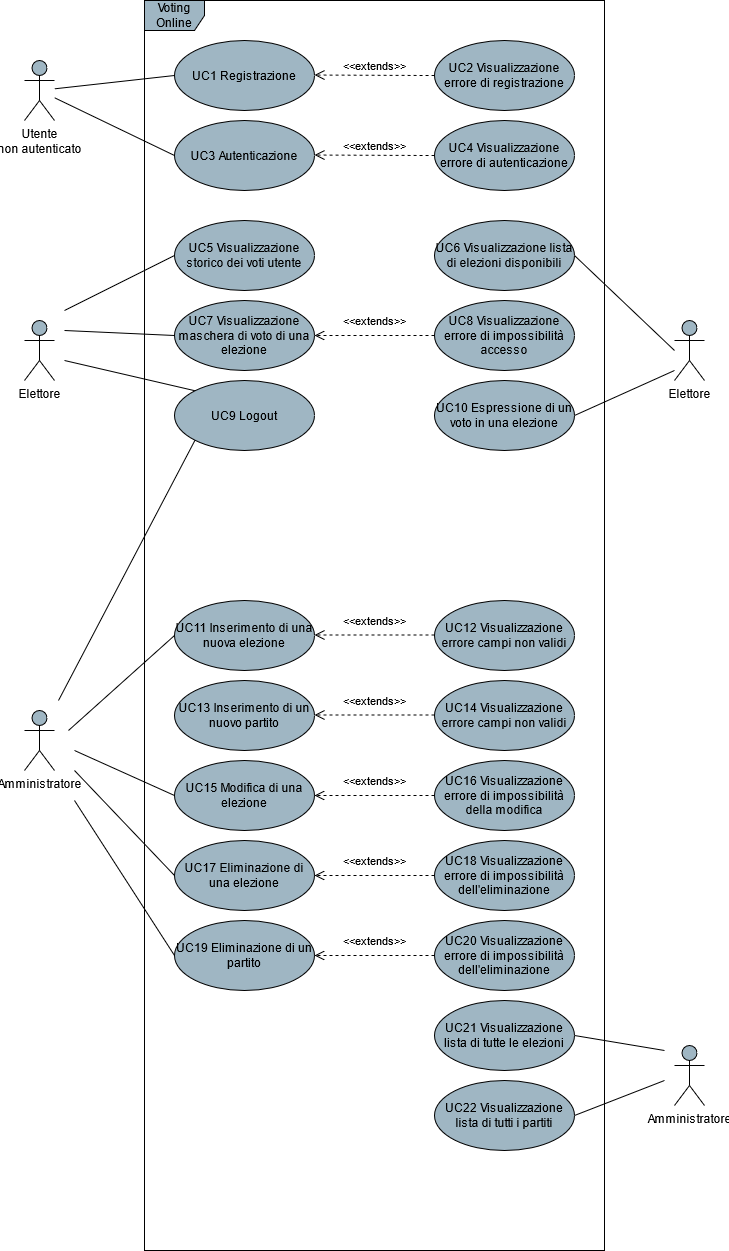
\includegraphics[width=0.9\columnwidth]{immagini/cap3/SchemaGenerale.png}
    \caption{Scenario principale}
\end{figure}

\clearpage

% ----------------------------------- UC1 ----------------------------------------------
\begin{usecase}{1}{Registrazione}
\usecaseactors{Utente non autenticato}
\usecasepre{L’utente non autenticato è all'interno della pagina di registrazione}
\usecasedesc{Viene effettuata la registrazione di un elettore nel sistema, inserendo i propri dati personali nella pagina dedicata}
\usecasescenario{L’utente non autenticato accede alla pagina di registrazione, il sistema rende disponibili i campi da compilare, l’utente inserisce l'indirizzo email [\textbf{UC1.1}], l'username [\textbf{UC1.2}], la password [\textbf{UC1.3}] e procede infine a confermare la registrazione}
\usecasepost{La registrazione nel sistema è avvenuta con successo} \\
\textbf{Estensioni:}
    \begin{enumerate}
        \item \textbf{UC2}: se i campi non sono validi o l'email è già stata utilizzata nel sistema, viene mostrato un errore di registrazione all'utente non autenticato che potrà provare nuovamente a ripetere la procedura.
    \end{enumerate}
\end{usecase}

\begin{figure}[!h] 
    \centering 
    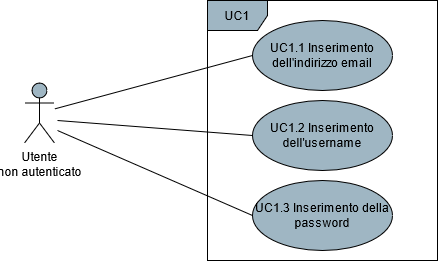
\includegraphics[width=0.9\columnwidth]{immagini/cap3/UC1.png} 
    \caption{Use Case - UC1: Registrazione}
\end{figure}

\begin{usecase}{1.1}{Inserimento dell'indirizzo email}
\usecaseactors{Utente non autenticato}
\usecasepre{Il campo “email” risulta vuoto}
\usecasedesc{L'utente deve compilare il campo “email” per procedere alla registrazione}
\usecasescenario{L'utente inserisce il suo indirizzo email nell'apposito campo}
\usecasepost{il campo “email” è stato compilato}
\end{usecase} \\ \\

\begin{usecase}{1.2}{Inserimento dell'username}
\usecaseactors{Utente non autenticato}
\usecasepre{Il campo “username” risulta vuoto}
\usecasedesc{L'utente deve compilare il campo “username” per procedere alla registrazione}
\usecasescenario{L'utente inserisce l'username desiderato nell'apposito campo}
\usecasepost{il campo “username” è stato compilato}
\end{usecase}

\begin{usecase}{1.3}{Inserimento della password}
\usecaseactors{Utente non autenticato}
\usecasepre{Il campo “password” risulta vuoto}
\usecasedesc{L'utente deve compilare il campo “password” per procedere alla registrazione}
\usecasescenario{L'utente inserisce la password desiderata nell'apposito campo}
\usecasepost{il campo “password” è stato compilato}
\end{usecase}

% ----------------------------------- UC2 ----------------------------------------------
\begin{usecase}{2}{Visualizzazione errore di registrazione}
\usecaseactors{Utente non autenticato}
\usecasepre{L'utente non autenticato ha inserito i campi ed ha provato ad effettuare
la registrazione}
\usecasedesc{L'utente non autenticato visualizza un errore riguardante i campi di registrazione che ha inserito} Questi errori possono essere:
    \begin{itemize}
        \item \textbf{campo non valido}: un campo risulta vuoto o con caratteri non validi;
        \item \textbf{email già utilizzata}: l'email è già stata utilizzata da un altro elettore.
    \end{itemize}
\usecasescenario{Il sistema riconosce uno o più errori nei campi inseriti dall'utente e vengono visualizzati nella pagina di registrazione}
\usecasepost{Viene visualizzato un messaggio di errore nella pagina di registrazione
e l’utente non risulta autenticato nel sistema} \\
\end{usecase}

% ----------------------------------- UC3 ----------------------------------------------
\begin{usecase}{3}{Autenticazione}
\usecaseactors{Utente non autenticato}
\usecasepre{L’utente non autenticato è all'interno della pagina di autenticazione}
\usecasedesc{L'utente non autenticato, inserendo le proprie credenziali, viene autenticato alla piattaforma}
\usecasescenario{L’utente non autenticato accede alla pagina di autenticazione, il sistema rende disponibili i campi da compilare, l’utente inserisce l'indirizzo email [\textbf{UC3.1}], la password [\textbf{UC3.2}] e procede infine inviando la richiesta}
\usecasepost{L'utente viene autenticato come elettore o amministratore dal sistema} \\
\textbf{Estensioni:}
    \begin{enumerate}
        \item \textbf{UC4}: se le credenziali inserite non vengono riconosciute dal sistema viene visualizzato un messaggio che informa l'utente dell'errore.
    \end{enumerate}
\end{usecase}

\begin{figure}[!h] 
    \centering 
    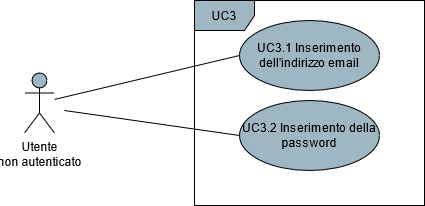
\includegraphics[width=0.9\columnwidth]{immagini/cap3/UC3.png} 
    \caption{Use Case - UC3: Autenticazione}
\end{figure}

\begin{usecase}{3.1}{Inserimento dell'indirizzo email}
\usecaseactors{Utente non autenticato}
\usecasepre{Il campo “email” risulta vuoto}
\usecasedesc{L'utente deve compilare il campo “email” per procedere all'autenticazione}
\usecasescenario{L'utente inserisce il proprio indirizzo email nell'apposito campo}
\usecasepost{il campo “email” è stato compilato}
\end{usecase}

\begin{usecase}{3.2}{Inserimento della password}
\usecaseactors{Utente non autenticato}
\usecasepre{Il campo “password” risulta vuoto}
\usecasedesc{L'utente deve compilare il campo “password” per procedere all'autenticazione}
\usecasescenario{L'utente inserisce la propria password nell'apposito campo}
\usecasepost{il campo “password” è stato compilato}
\end{usecase} \\

% ----------------------------------- UC4 ----------------------------------------------
\begin{usecase}{4}{Visualizzazione errore di autenticazione}
\usecaseactors{Utente non autenticato}
\usecasepre{L'utente non autenticato ha inserito i campi ed ha provato ad effettuare
l'autenticazione}
\usecasedesc{L'utente non autenticato visualizza un messaggio di errore che lo informa che i dati da lui inseriti durante il login non sono riconosciuti dal sistema}
\usecasescenario{:L'utente tenta di effettuare il login usando credenziali non presenti nel sistema}
\usecasepost{Viene visualizzato un messaggio di errore nella pagina di autenticazione
e l’utente non risulta autenticato nel sistema} \\
\end{usecase}

% ----------------------------------- UC5 ----------------------------------------------
\begin{usecase}{5}{Visualizzazione storico dei voti dei voti dell'utente}
\usecaseactors{Elettore}
\usecasepre{L’elettore è all'interno della pagina corrispondente alla sua dashboard personale}
\usecasedesc{L'elettore può visualizzare, nel caso abbia partecipato ad almeno un'elezione, lo storico dei propri voti}
\usecasescenario{L’elettore può visualizzare lo storico dei propri voti nella forma di una lista di singole votazioni passate [\textbf{UC5.1}]}
\usecasepost{L'elettore visualizza lo storico dei voti}
\end{usecase}

\begin{figure}[!h] 
    \centering 
    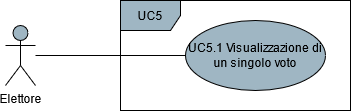
\includegraphics[width=0.9\columnwidth]{immagini/cap3/UC5.png} 
    \caption{Use Case - UC5: Visualizzazione storico dei voti dei voti dell'utente}
\end{figure}

\begin{usecase}{5.1}{Visualizzazione di un singolo voto}
\usecaseactors{Elettore}
\usecasepre{L’elettore è all'interno della pagina corrispondente alla sua dashboard personale}
\usecasedesc{L'elettore può visualizzare le informazioni corrispondenti ad un singolo voto appartenente al suo storico}
\usecasescenario{L'elettore visualizza le seguenti informazioni caratterizzanti di un voto appartenente al suo storico: il nome dell'elezione, la data di inizio e di fine dell'elezione, di espressione del voto, il partito e il candidato votato}
\usecasepost{L'elettore visualizza tutti i dati che caratterizzano un suo voto passato}
\end{usecase}

% ----------------------------------- UC6 ----------------------------------------------
\begin{usecase}{6}{Visualizzazione lista delle elezioni disponibili}
\usecaseactors{Elettore}
\usecasepre{L’elettore è all'interno della pagina corrispondente alla sua dashboard personale}
\usecasedesc{L'elettore può visualizzare, nel caso sia presente almeno un'elezione aperta nella data corrente, un elenco di elezioni}
\usecasescenario{L’elettore può visualizzare le elezioni disponibili nella forma di una lista di singole votazioni [\textbf{UC6.1}]}
\usecasepost{L'elettore visualizza le elezioni disponibili nella dashboard personale}
\end{usecase}

\begin{figure}[!h] 
    \centering 
    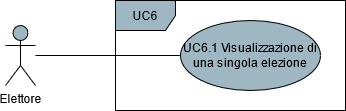
\includegraphics[width=0.9\columnwidth]{immagini/cap3/UC6.png} 
    \caption{Use Case - UC6: Visualizzazione lista delle elezioni disponibili}
\end{figure}

\begin{usecase}{6.1}{Visualizzazione di una singola elezione}
\usecaseactors{Elettore}
\usecasepre{L’elettore è all'interno della pagina corrispondente alla sua dashboard personale}
\usecasedesc{L'elettore può visualizzare le informazioni corrispondenti ad una singola elezione presente nell'elenco delle elezioni disponibili}
\usecasescenario{L'elettore visualizza le seguenti informazioni caratterizzanti di un'elezione disponibile: il nome, la tipologia, la data di inizio e di fine della votazione}
\usecasepost{L'elettore visualizza tutti i dati che caratterizzano una singola elezione disponibile}
\end{usecase}

% ----------------------------------- UC7 ----------------------------------------------
\begin{usecase}{7}{Visualizzazione maschera di voto di una elezione}
\usecaseactors{Elettore}
\usecasepre{L’elettore visualizza l'elenco delle elezioni disponibili ed è presente almeno una voce nella lista}
\usecasedesc{L'elettore accede alla maschera di voto per esprimere la propria preferenza cliccando su un'elezione disponibile, rispetto alla quale visualizzerà le informazioni nececessarie per procedere alla votazione}
\usecasescenario{L’elettore, cliccando su una delle elezioni disponibili nella lista [\textbf{UC6}], accede alla maschera di voto di tale elezione, della quale visualizza il relativo nome, le istruzioni per esprimere la propria preferenza con successo e la lista dei partiti partecipanti [\textbf{UC7.1}]}
\usecasepost{L'elettore visualizza le informazioni necessarie per esprimere il proprio voto nell'apposita pagina}
\textbf{Estensioni:}
    \begin{enumerate}
        \item \textbf{UC8}: se si clicca su un'elezione per la quale l'elettore ha già espresso una preferenza viene visualizzato un messaggio che avvisa l'utente dell'errore.
    \end{enumerate}
\end{usecase}

\begin{figure}[!h] 
    \centering 
    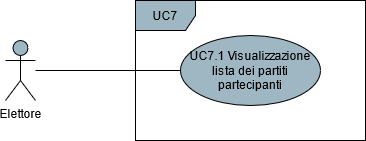
\includegraphics[width=0.9\columnwidth]{immagini/cap3/UC7.png} 
    \caption{Use Case - UC7: Visualizzazione maschera di voto di una elezione}
\end{figure}

\begin{usecase}{7.1}{Visualizzazione lista dei partiti partecipanti}
\usecaseactors{Elettore}
\usecasepre{L’elettore è all'interno della pagina corrispondente alla maschera di voto per una elezione}
\usecasedesc{L'elettore può visualizzare, nel caso sia presente almeno un partito partecipante, una lista di partiti}
\usecasescenario{L’elettore può visualizzare i partiti partecipanti nella forma di una lista di singoli partiti [\textbf{UC7.1.1}]}
\usecasepost{L'elettore visualizza tutti i partiti partecipanti che possono essere votati nella maschera di voto relativa ad una specifica elezione}
\end{usecase} \\

\begin{figure}[!h] 
    \centering 
    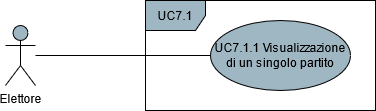
\includegraphics[width=0.9\columnwidth]{immagini/cap3/UC7_1.png} 
    \caption{Use Case - UC7.1: Visualizzazione lista dei partiti partecipanti}
\end{figure}

\begin{usecase}{7.1.1}{Visualizzazione di un singolo partito}
\usecaseactors{Elettore}
\usecasepre{L’elettore è all'interno della pagina corrispondente alla maschera di voto per una elezione e sta visualizzando la lista dei partiti partecipanti}
\usecasedesc{L'elettore può visualizzare le informazioni corrispondenti ad un singolo partito presente nell'elenco dei partiti partecipanti}
\usecasescenario{L'elettore visualizza le seguenti informazioni caratterizzanti del partito partecipante: il logo, il nome e il nominativo del candidato associato al partito}
\usecasepost{L'elettore visualizza tutti i dati che caratterizzano un singolo partito partecipante all'elezione}
\end{usecase}

% ----------------------------------- UC8 ----------------------------------------------
\begin{usecase}{8}{Visualizzazione errore di impossibilità di accesso all'elezione}
\usecaseactors{Elettore}
\usecasepre{L’elettore visualizza l'elenco delle elezioni disponibili ed ha provato a cliccare su una delle voci presenti nella lista}
\usecasedesc{L'elettore visualizza un messaggio di errore riguardante l'impossibilità di accedere alla maschera di voto relativa all'elezione selezionata. Questo errore indica che è stata già effettuata una preferenza per questa elezione}
\usecasescenario{Il sistema riconosce un errore al tentativo di accesso da parte dell'elettore ad un'elezione e viene visualizzato il relativo messaggio di errore nella dashboard personale}
\usecasepost{Viene visualizzato un messaggio di errore nella dashboard personale dell'elettore e quest'ultimo non ha la possibilità di accedere alla maschera di voto relativa all'elezione selezionata} \\
\end{usecase}

% ----------------------------------- UC9 ----------------------------------------------
\begin{usecase}{9}{Logout}
\usecaseactors{Elettore, Amministratore}
\usecasepre{L'utente, che ha precedentemente effettuato la procedura di login, è attualmente autenticato nella piattaforma}
\usecasedesc{Viene effettuato il logout di un'utente autenticato, che può essere un elettore o amministratore}
\usecasescenario{L'utente richiede il logout tramite un bottone dedicato}
\usecasepost{L'utente non è più autenticato nel sistema} \\ \\
\end{usecase}

% ----------------------------------- UC10 ----------------------------------------------
\begin{usecase}{10}{Espressione di un voto in un'elezione}
\usecaseactors{Elettore}
\usecasepre{L’elettore si trova nella pagina relativa alla maschera di voto di una specifica elezione}
\usecasedesc{L'elettore può esprimere il proprio voto in una determinata elezione selezionando il partito desiderato e confermando infine la propria scelta}
\usecasescenario{L'elettore, visualizzando le informazioni contenute nella maschera di voto [\textbf{UC7}] dell'elezione in questione, può procedere ad esprimere la propria preferenza selezionando uno tra i partiti partecipanti [\textbf{UC10.1}] e confermando successivamente la propria decisione [\textbf{UC10.2}]}
\usecasepost{L'elettore ha votato per un partito partecipante ad una specifica elezione}
\end{usecase}

\begin{figure}[!h] 
    \centering
    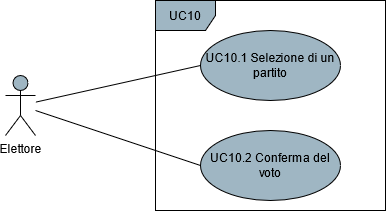
\includegraphics[width=0.9\columnwidth]{immagini/cap3/UC10.png} 
    \caption{Use Case - UC10: Espressione di un voto in un'elezione}
\end{figure}

\begin{usecase}{10.1}{Selezione di un partito}
\usecaseactors{Elettore}
\usecasepre{L’elettore si trova nella pagina relativa alla maschera di voto di una specifica elezione}
\usecasedesc{L'elettore deve selezionare esattamente un partito dalla lista dei partiti partecipanti per poter continuare con la procedura di voto}
\usecasescenario{L'elettore, visualizzando la lista di partiti partecipanti contenuta nella maschera di voto [\textbf{UC7.1}] dell'elezione in questione, deve selezionare esattamente uno tra i partiti partecipanti per esprimere la propria preferenza}
\usecasepost{L'elettore ha selezionato un partito partecipante all'elezione in questione} \\ \\
\end{usecase}

\begin{usecase}{10.2}{Conferma del voto}
\usecaseactors{Elettore}
\usecasepre{L’elettore si trova nella pagina relativa alla maschera di voto di una specifica elezione ed ha selezionato un partito partecipante}
\usecasedesc{L'elettore deve confermare il partito scelto come preferenza per concludere la votazione}
\usecasescenario{L'elettore, dopo aver selezionato un partito partecipante come preferenza [\textbf{UC10.1}], deve cliccare sull'apposito pulsante per richiedere la conclusione della votazione e, visualizzando un apposito riquadro di riepilogo, deve confermare la propria decisione per concludere la procedura di voto}
\usecasepost{L'elettore ha confermato la preferenza del partito partecipante scelto all'elezione in questione}
\end{usecase}

% ----------------------------------- UC11 ----------------------------------------------
\begin{usecase}{11}{Inserimento di una nuova elezione}
\usecaseactors{Amministratore}
\usecasepre{L’amministratore si trova nella pagina corrispondente alla admin dashboard}
\usecasedesc{L'amministratore può inserire una nuova elezione nella piattaforma inserendo gli appositi dati}
\usecasescenario{L'amministratore per inserire una nuova elezione deve compilare i campi dati in modo da descriverne le seguenti informazioni: il nome [\textbf{UC11.1}], la tipologia [\textbf{UC11.2}], la data di inizio [\textbf{UC11.3}] e di fine [\textbf{UC11.4}]. E' necessario, infine, che vengano selezionati i partiti partecipanti da un apposito elenco [\textbf{UC11.5}]}
\usecasepost{L'amministratore ha inserito una nuova elezione nel sistema con successo} \\
\textbf{Estensioni:}
    \begin{enumerate}
        \item \textbf{UC12}: se i campi non sono validi viene mostrato un errore di inserimento all'amministratore che potrà provare nuovamente a ripetere la procedura modificando i campi che hanno causato l'errore.
    \end{enumerate}
\end{usecase}

\begin{figure}[!h] 
    \centering
    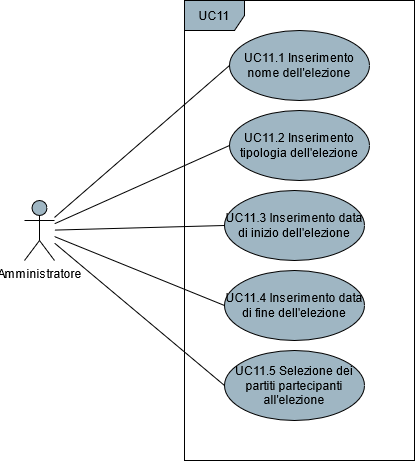
\includegraphics[width=0.9\columnwidth]{immagini/cap3/UC11.png} 
    \caption{Use Case - UC11: Inserimento di una nuova elezione}
\end{figure}

\begin{usecase}{11.1}{Inserimento del nome}
\usecaseactors{Amministratore}
\usecasepre{Il campo “nome” risulta vuoto}
\usecasedesc{L'amministratore deve compilare il campo “nome” per procedere all'inserimento}
\usecasescenario{L'amministratore inserisce il nome dell'elezione nell'apposito campo}
\usecasepost{il campo “nome” è stato compilato}
\end{usecase}

\begin{usecase}{11.2}{Inserimento della tipologia}
\usecaseactors{Amministratore}
\usecasepre{Il campo “tipologia” risulta vuoto}
\usecasedesc{L'amministratore deve compilare il campo “tipologia” per procedere all'inserimento}
\usecasescenario{L'amministratore inserisce la tipologia dell'elezione nell'apposito campo}
\usecasepost{il campo “tipologia” è stato compilato}
\end{usecase}

\begin{usecase}{11.3}{Inserimento della data di inizio}
\usecaseactors{Amministratore}
\usecasepre{Il campo “data di inizio” risulta vuoto}
\usecasedesc{L'amministratore deve compilare il campo “data di inizio” per procedere all'inserimento}
\usecasescenario{L'amministratore inserisce la data di inizio dell'elezione nell'apposito campo}
\usecasepost{il campo “data di inizio” è stato compilato}
\end{usecase}

\begin{usecase}{11.4}{Inserimento della data di fine}
\usecaseactors{Amministratore}
\usecasepre{Il campo “data di fine” risulta vuoto}
\usecasedesc{L'amministratore deve compilare il campo “data di fine” per procedere all'inserimento}
\usecasescenario{L'amministratore inserisce la data di fine dell'elezione nell'apposito campo}
\usecasepost{il campo “data di fine” è stato compilato}
\end{usecase}

\begin{usecase}{11.5}{Selezione dei partiti partecipanti all'elezione}
\usecaseactors{Amministratore}
\usecasepre{Nessun partito risulta selezionato nell'elenco dei partiti partecipanti}
\usecasedesc{L'amministratore può decidere di selezionare nessuno o tutti i partiti presenti nel sistema in modo da renderli partecipanti all'elezione. La selezione dei partiti partecipanti è modificabile in seguito utilizzando la funzionalità di modifica dell'elezione [\textbf{UC15}]}
\usecasescenario{L'amministratore decide quali partiti aggiungere all'elezione in questione selezionandoli nell'apposito elenco che contiene tutti i partiti presenti nella piattaforma}
\usecasepost{L'elenco dei partiti partecipanti è stato compilato da parte dell'amministratore}
\end{usecase}

% ----------------------------------- UC12 ----------------------------------------------
\begin{usecase}{12}{Visualizzazione errore per campi non validi}
\usecaseactors{Amministratore}
\usecasepre{L'amministratore ha compilato i campi ed ha provato ad effettuare l'inserimento di una nuova elezione}
\usecasedesc{L'amministratore visualizza un errore riguardante uno o più campi che ha compilato e che risultano invalidi perchè vuoti o perchè c'è un errore nella formattazione del contenuto}
\usecasescenario{Il sistema riconosce uno o più errori nei campi inseriti dall'amministratore e vengono visualizzati nell'apposita form di inserimento}
\usecasepost{Viene visualizzato un messaggio di errore nella form e la nuova elezione non risulta inserita nel sistema} \\
\end{usecase}

% ----------------------------------- UC13 ----------------------------------------------
\begin{usecase}{13}{Inserimento di un nuovo partito}
\usecasepre{L’amministratore si trova nella pagina corrispondente alla admin dashboard}
\usecasedesc{L'amministratore può inserire un nuovo partito nella piattaforma inserendo gli appositi dati}
\usecasescenario{L'amministratore per inserire un nuovo partito deve compilare i campi dati in modo da descriverne le seguenti caratteristiche: il nome [\textbf{UC13.1}] e il nominativo del candidato [\textbf{UC13.2}]. E' necessario, infine, che venga inserito il logo del partito in formato immagine (PNG/JPEG) [\textbf{UC13.3}]}
\usecasepost{L'amministratore ha inserito un nuovo partito nel sistema con successo} \\
\textbf{Estensioni:}
    \begin{enumerate}
        \item \textbf{UC14}: se i campi non sono validi viene mostrato un errore di inserimento all'amministratore che potrà provare nuovamente a ripetere la procedura modificando i campi che hanno causato l'errore.
    \end{enumerate}
\end{usecase}

\begin{figure}[!h] 
    \centering
    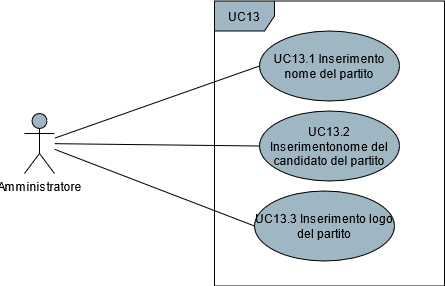
\includegraphics[width=0.9\columnwidth]{immagini/cap3/UC13.png} 
    \caption{Use Case - UC13: Inserimento di un nuovo partito}
\end{figure}

\begin{usecase}{13.1}{Inserimento del nome}
\usecaseactors{Amministratore}
\usecasepre{Il campo “nome” risulta vuoto}
\usecasedesc{L'amministratore deve compilare il campo “nome” per procedere all'inserimento}
\usecasescenario{L'amministratore inserisce il nome del partito nell'apposito campo}
\usecasepost{il campo “nome” è stato compilato}
\end{usecase}

\begin{usecase}{13.2}{Inserimento del candidato}
\usecaseactors{Amministratore}
\usecasepre{Il campo “candidato” risulta vuoto}
\usecasedesc{L'amministratore deve compilare il campo “candidato” inserendo il nominativo del candidato per il partito in modo da procedere all'inserimento}
\usecasescenario{L'amministratore inserisce il nominativo del candidato del partito nell'apposito campo}
\usecasepost{il campo “candidato” è stato compilato}
\end{usecase}

\begin{usecase}{13.3}{Inserimento del logo}
\usecaseactors{Amministratore}
\usecasepre{Il campo nel quale inserire il logo del partito risulta vuoto}
\usecasedesc{L'amministratore deve inserire il logo del partito in formato immagine (PNG/JPEG) per procedere all'inserimento}
\usecasescenario{L'amministratore inserisce il logo del partito nell'apposito campo}
\usecasepost{Il logo del partito è stato inserito nell'apposito campo}
\end{usecase}

% ----------------------------------- UC14 ----------------------------------------------
\begin{usecase}{14}{Visualizzazione errore per campi non validi}
\usecaseactors{Amministratore}
\usecasepre{L'amministratore ha compilato i campi ed ha provato ad effettuare l'inserimento di un nuovo partito}
\usecasedesc{L'amministratore visualizza un errore riguardante uno o più campi che ha compilato e che risultano invalidi perchè vuoti o perchè c'è un errore nella formattazione del contenuto}
\usecasescenario{Il sistema riconosce uno o più errori nei campi inseriti dall'amministratore e vengono visualizzati nell'apposita form di inserimento}
\usecasepost{Viene visualizzato un messaggio di errore nella form e il nuovo partito non risulta inserito nel sistema}
\end{usecase}

% ----------------------------------- UC15 ----------------------------------------------
\begin{usecase}{15}{Modifica di una elezione}
\usecaseactors{Amministratore}
\usecasepre{L’amministratore si trova nella pagina corrispondente alla admin dashboard e visualizza le informazioni di dettaglio di un'elezione}
\usecasedesc{L'amministratore può modificare un'elezione presente nella piattaforma compilando gli appositi campi dati}
\usecasescenario{L'amministratore per modificare un'elezione esistente deve, rendendo editabili le sue informazioni attraverso l'apposito pulsante, compilare i campi dati in modo da descrivere almeno una delle seguenti informazioni: il nome [\textbf{UC15.1}], la tipologia [\textbf{UC15.2}], la data di inizio [\textbf{UC15.3}] e di fine [\textbf{UC15.4}]. E' possibile, inoltre, modificare i partiti partecipanti alterando le voci selezionate di un apposito elenco [\textbf{UC15.5}] e, infine, la modifica deve essere confermata da un apposito pulsante}
\usecasepost{L'amministratore ha modificato un'elezione presente nel sistema con successo} \\
\textbf{Estensioni:}
    \begin{enumerate}
        \item \textbf{UC16}: nel caso in cui un'elezione risulti cominciata o già terminata non è possibile modificarla, verrà quindi mostrato un messaggio esplicativo all'amministratore, il quale non potrà procedere con la modifica.
    \end{enumerate}
\end{usecase}

\begin{figure}[!h] 
    \centering
    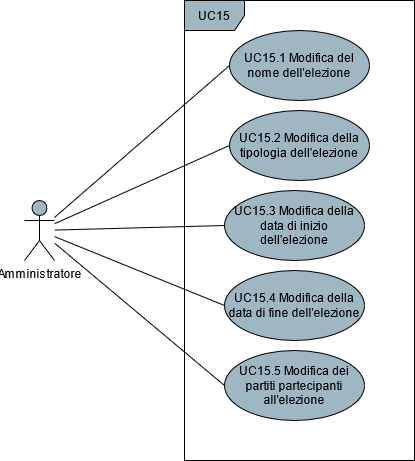
\includegraphics[width=0.9\columnwidth]{immagini/cap3/UC15.png} 
    \caption{Use Case - UC15: Modifica di una elezione}
\end{figure}

\begin{usecase}{15.1}{Modifica del nome}
\usecaseactors{Amministratore}
\usecasepre{Il campo “nome” risulta occupato dall'informazione attuale dell'elezione}
\usecasedesc{L'amministratore può compilare il campo “nome” per procedere alla modifica di tale informazione}
\usecasescenario{L'amministratore inserisce il nuovo nome dell'elezione nell'apposito campo}
\usecasepost{il campo “nome” è stato modificato}
\end{usecase}

\begin{usecase}{15.2}{Modifica della tipologia}
\usecaseactors{Amministratore}
\usecasepre{Il campo “tipologia” risulta occupato dall'informazione attuale dell'elezione}
\usecasedesc{L'amministratore può compilare il campo “tipologia” per procedere alla modifica di tale informazione}
\usecasescenario{L'amministratore inserisce la nuova tipologia dell'elezione nell'apposito campo}
\usecasepost{il campo “tipologia” è stato modificato}
\end{usecase}

\begin{usecase}{15.3}{Modifica della data di inizio}
\usecaseactors{Amministratore}
\usecasepre{Il campo “data di inizio” risulta occupato dall'informazione attuale dell'elezione}
\usecasedesc{L'amministratore può compilare il campo “data di inizio” per procedere alla modifica di tale informazione}
\usecasescenario{L'amministratore inserisce la nuova data di inizio dell'elezione nell'apposito campo}
\usecasepost{il campo “data di inizio” è stato modificato}
\end{usecase}

\begin{usecase}{15.4}{Modifica della data di fine}
\usecaseactors{Amministratore}
\usecasepre{Il campo “data di fine” risulta occupato dall'informazione attuale dell'elezione}
\usecasedesc{L'amministratore può compilare il campo “data di fine” per procedere alla modifica di tale informazione}
\usecasescenario{L'amministratore inserisce la nuova data di fine dell'elezione nell'apposito campo}
\usecasepost{il campo “data di fine” è stato modificato}
\end{usecase}

\begin{usecase}{15.5}{Modifica dei partiti partecipanti all'elezione}
\usecaseactors{Amministratore}
\usecasepre{L'elenco dei partiti partecipanti contiene le informazioni attuali riguardo ai partiti}
\usecasedesc{L'amministratore può decidere di modificare l'elenco selezionando nessuno o tutti i partiti presenti nel sistema in modo da renderli partecipanti all'elezione. La selezione dei partiti partecipanti è modificabile finché non arriva la data di inizio dell'elezione}
\usecasescenario{L'amministratore decide quali partiti aggiungere o rimuovere dall'elezione in questione selezionandoli nell'apposito elenco che contiene tutti i partiti presenti nella piattaforma}
\usecasepost{L'elenco dei partiti partecipanti è stato modificato da parte dell'amministratore}
\end{usecase}

% ----------------------------------- UC16 ----------------------------------------------
\begin{usecase}{16}{Visualizzazione errore per impossibilità della modifica}
\usecaseactors{Amministratore}
\usecasepre{L'amministratore visualizza le informazioni riguardanti un'elezione già cominciata o conclusa ed ha provato a cliccare sul pulsante per abilitare la loro modifica}
\usecasedesc{Viene mostrato all'amministratore un messaggio che indica che non è possibile modificare un'elezione già cominciata o conclusa}
\usecasescenario{Il sistema mostra un messaggio esplicativo dell'errore all'amministratore}
\usecasepost{Viene visualizzato un messaggio di errore nella admin dashboard e non viene permessa la modifica dell'elezione all'amministratore} \\
\end{usecase}

% ----------------------------------- UC17 ----------------------------------------------
\begin{usecase}{17}{Eliminazione di una elezione}
\usecaseactors{Amministratore}
\usecasepre{L’amministratore si trova nella pagina corrispondente alla admin dashboard e visualizza le informazioni di dettaglio di un'elezione}
\usecasedesc{L'amministratore può eliminare un'elezione presente nella piattaforma cliccando l'apposito pulsante}
\usecasescenario{L'amministratore per eliminare un'elezione esistente deve premere l'apposito pulsante situato contestualmente alle informazioni dell'elezione stessa}
\usecasepost{L'amministratore ha eliminato un'elezione presente nel sistema con successo} \\
\textbf{Estensioni:}
    \begin{enumerate}
        \item \textbf{UC18}: nel caso in cui un'elezione risulti cominciata o già terminata non è possibile eliminarla, verrà quindi mostrato un messaggio esplicativo all'amministratore, il quale non potrà procedere con l'eliminazione.
    \end{enumerate}
\end{usecase}

% ----------------------------------- UC18 ----------------------------------------------
\begin{usecase}{18}{Visualizzazione errore per impossibilità dell'eliminazione}
\usecaseactors{Amministratore}
\usecasepre{L'amministratore visualizza le informazioni riguardanti un'elezione già cominciata o conclusa ed ha provato a cliccare sul pulsante per eliminarla}
\usecasedesc{Viene mostrato all'amministratore un messaggio che indica che non è possibile eliminare un'elezione già cominciata o conclusa}
\usecasescenario{Il sistema mostra un messaggio esplicativo dell'errore all'amministratore}
\usecasepost{Viene visualizzato un messaggio di errore nella admin dashboard e non viene permessa l'eliminazione dell'elezione all'amministratore} \\
\end{usecase}

% ----------------------------------- UC19 ----------------------------------------------
\begin{usecase}{19}{Eliminazione di un partito}
\usecaseactors{Amministratore}
\usecasepre{L’amministratore si trova nella pagina corrispondente alla admin dashboard e visualizza le informazioni di dettaglio di un partito}
\usecasedesc{L'amministratore può eliminare un partito presente nella piattaforma cliccando l'apposito pulsante}
\usecasescenario{L'amministratore per eliminare un partito esistente deve premere l'apposito pulsante situato contestualmente alle informazioni del partito stesso}
\usecasepost{L'amministratore ha eliminato un partito dal sistema con successo} \\
\textbf{Estensioni:}
    \begin{enumerate}
        \item \textbf{UC20}: nel caso in cui un partito risulti presente in un'elezione già cominciata o terminata non è possibile eliminarlo, verrà quindi mostrato un messaggio esplicativo all'amministratore, il quale non potrà procedere con l'eliminazione.
    \end{enumerate}
\end{usecase}

% ----------------------------------- UC20 ----------------------------------------------
\begin{usecase}{20}{Visualizzazione errore per impossibilità dell'eliminazione}
\usecaseactors{Amministratore}
\usecasepre{L'amministratore visualizza le informazioni riguardanti un partito partecipante in un'elezione già cominciata o conclusa ed ha provato a cliccare sul pulsante per eliminarlo}
\usecasedesc{Viene mostrato all'amministratore un messaggio che indica che non è possibile eliminare un partito facente parte di un'elezione già cominciata o conclusa}
\usecasescenario{Il sistema mostra un messaggio esplicativo dell'errore all'amministratore}
\usecasepost{Viene visualizzato un messaggio di errore nella admin dashboard e non viene permessa l'eliminazione del partito all'amministratore}
\end{usecase}

% ----------------------------------- UC21 ----------------------------------------------
\begin{usecase}{21}{Visualizzazione lista di tutte le elezioni}
\usecaseactors{Amministratore}
\usecasepre{L’amministratore è all'interno della pagina corrispondente all'admin dashboard}
\usecasedesc{L'amministratore può visualizzare, nel caso sia stata inserita nella piattaforma almeno un'elezione, un elenco di elezioni}
\usecasescenario{L’amministratore può visualizzare tutte le elezioni precedentemente inserite nella piattaforma con la forma di una lista di singole votazioni [\textbf{UC21.1}]}
\usecasepost{L'amministratore visualizza le elezioni presenti nella piattaforma sulla admin dashboard}
\end{usecase}

\begin{figure}[!h] 
    \centering 
    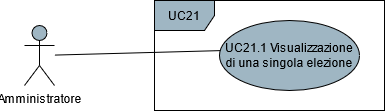
\includegraphics[width=0.9\columnwidth]{immagini/cap3/UC21.png} 
    \caption{Use Case - UC21: Visualizzazione lista di tutte le elezioni}
\end{figure}

\begin{usecase}{21.1}{Visualizzazione di una singola elezione}
\usecaseactors{Amministratore}
\usecasepre{L'amministratore è all'interno della pagina corrispondente all'admin dashboard}
\usecasedesc{L'amministratore può visualizzare le informazioni corrispondenti ad una singola elezione presente nell'elenco di tutte le elezioni}
\usecasescenario{L'amministratore visualizza le seguenti informazioni caratterizzanti di un'elezione: il nome, la tipologia, la data di inizio e di fine della votazione}
\usecasepost{L'amministratore visualizza tutti i dati che caratterizzano una singola elezione}
\end{usecase}

% ----------------------------------- UC22 ----------------------------------------------
\begin{usecase}{22}{Visualizzazione lista di tutti i partiti}
\usecaseactors{Amministratore}
\usecasepre{L’amministratore è all'interno della pagina corrispondente all'admin dashboard}
\usecasedesc{L'amministratore può visualizzare, nel caso sia stato inserito nella piattaforma almeno un partito, un elenco di partiti}
\usecasescenario{L’amministratore può visualizzare tutti i partiti precedentemente inseriti nella piattaforma con la forma di una lista di singoli partiti [\textbf{UC22.1}]}
\usecasepost{L'amministratore visualizza tutti i partiti presenti nella piattaforma sulla admin dashboard}
\end{usecase}

\begin{figure}[!h] 
    \centering 
    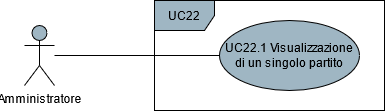
\includegraphics[width=0.9\columnwidth]{immagini/cap3/UC22.png} 
    \caption{Use Case - UC22: Visualizzazione lista di tutti i partiti}
\end{figure}

\begin{usecase}{22.1}{Visualizzazione di un singolo partito}
\usecaseactors{Amministratore}
\usecasepre{L'amministratore è all'interno della pagina corrispondente all'admin dashboard}
\usecasedesc{L'amministratore può visualizzare le informazioni che caratterizzano un singolo partito presente nell'elenco di tutti i partiti}
\usecasescenario{L'amministratore visualizza le seguenti informazioni caratterizzanti di un'elezione disponibile: il nome, il logo e il nominativo del candidato del partito}
\usecasepost{L'amministratore visualizza tutti i dati che caratterizzano un singolo partito}
\end{usecase}

% ----------------------------- TRACCIAMENTO REQUISITI --------------------------------------

\section{Tracciamento dei requisiti}

Da un'attenta analisi dei requisiti e degli use case effettuata sul progetto è stata stilata la tabella che traccia i requisiti in rapporto agli use case.\\
Sono stati individuati diversi tipi di requisiti e si è quindi fatto utilizzo di un codice identificativo per distinguerli.\\
Il codice dei requisiti è così strutturato R(F/Q/V)(N/D/O) dove:
\begin{enumerate}
	\item[R =] requisito
    \item[F =] funzionale
    \item[Q =] qualitativo
    \item[V =] di vincolo
    \item[N =] obbligatorio (necessario)
    \item[D =] desiderabile
    \item[Z =] opzionale
\end{enumerate}
Le fonti dei requisiti possono essere le seguenti:
\begin{itemize}
    \item UC[numero]: indica un caso d'uso;
    \item Committente: indica il capo progetto.
\end{itemize}
Nelle tabelle \ref{tab:requisiti-funzionali}, \ref{tab:requisiti-qualitativi} e \ref{tab:requisiti-vincolo} sono riassunti i requisiti e il loro tracciamento con gli use case delineati in fase di analisi.

\newpage

%\begin{table}%
%\caption{Tabella del tracciamento dei requisti funzionali}
%\label{tab:requisiti-funzionali}
%\begin{tabularx}{\textwidth}{lXl}
\begin{longtable}{| p{.20\textwidth} | p{.60\textwidth} | p{.20\textwidth} |}
\caption{Tabella del tracciamento dei requisti funzionali}
\label{tab:requisiti-funzionali}
\hline

\textbf{Requisito} & \textbf{Descrizione} & \textbf{Fonte}\\

\hline

RFN-1     & Il sistema deve permettere la registrazione di un nuovo elettore & UC1 \\

\hline

RFN-1.1     & Il sistema deve permettere l'inserimento dell'indirizzo email in fase di registrazione & UC1.1 \\

\hline

RFN-1.2     & Il sistema deve permettere l'inserimento dell'username in fase di registrazione & UC1.2 \\

\hline

RFN-1.3     & Il sistema deve permettere l'inserimento della password in fase di registrazione & UC1.3 \\

\hline

RFN-2     & Il sistema deve mostrare un errore nel caso in cui i campi non siano validi in fase di registrazione & UC2 \\

\hline

RFN-3     & Il sistema deve permettere l'autenticazione di un utente registrato come elettore o amministratore & UC3 \\

\hline

RFN-3.1     & Il sistema deve permettere l'inserimento dell'indirizzo email in fase di autenticazione & UC3.1 \\

\hline

RFN-3.2     & Il sistema deve permettere l'inserimento della password in fase di autenticazione & UC3.2 \\

\hline

RFN-4     & Il sistema deve mostrare un errore nel caso in cui i dati inseriti negli appositi campi non vengano riconosciuti in fase di autenticazione & UC4 \\

\hline

RFN-5     & Il sistema deve permettere di visualizzare lo storico dei voti ad un elettore & UC5 \\

\hline

RFN-5.1     & Il sistema deve permettere di visualizzare le informazioni di ogni singolo voto appartenente allo storico di un elettore & UC5.1 \\

\hline

RFN-6     & Il sistema deve permettere di visualizzare tutte le elezioni disponibili ad un elettore & UC6 \\

\hline

RFN-6.1     & Il sistema deve permettere di visualizzare le informazioni di ogni singola votazione appartenente alle elezioni disponibili di un elettore & UC6.1 \\

\hline

RFN-7     & Il sistema deve permettere di visualizzare la maschera di voto di una specifica elezione ad un elettore & UC7 \\

\hline

RFN-7.1     & Il sistema deve permettere di visualizzare la lista dei partiti partecipanti nella maschera di voto di una specifica elezione & UC7.1 \\

\hline

RFN-7.1.1     & Il sistema deve permettere di visualizzare le informazioni di ogni singolo partito partecipante nella maschera di voto di una specifica elezione & UC7.1.1 \\

\hline

RFN-8     & Il sistema deve mostrare un errore nel caso in cui l'elettore provi ad accedere alla maschera di voto di un'elezione per la quale ha già espresso il proprio voto & UC8 \\

\hline

RFN-9     & Il sistema deve permettere l'uscita dalla piattaforma da parte di un utente precedentemente auteticato come elettore o amministratore & UC9 \\

\hline

RFN-10     & Il sistema deve permettere ad un elettore l'espressione della propria preferenza all'interno della maschera di voto di una specifica elezione  & UC10 \\

\hline

RFN-10.1     & Il sistema deve permettere ad un elettore di selezionare esattamente un partito dalla lista dei partiti partecipanti nella maschera di voto  & UC10.1 \\

\hline

RFD-10.2     & Il sistema deve permettere ad un elettore di confermare la scelta del partito selezionato, visualizzando un riquadro di riepilogo  & UC10.2 \\

\hline

RFN-11     & Il sistema deve permettere ad un amministratore l'inserimento di una nuova elezione nella piattaforma  & UC11 \\

\hline

RFN-11.1     & Il sistema deve permettere ad un amministratore l'inserimento del nome in fase di inserimento di una nuova elezione  & UC11.1 \\

\hline

RFN-11.2     & Il sistema deve permettere ad un amministratore l'inserimento della tipologia in fase di inserimento di una nuova elezione  & UC11.2 \\

\hline

RFN-11.3     & Il sistema deve permettere ad un amministratore l'inserimento della data di inizio in fase di inserimento di una nuova elezione  & UC11.3 \\

\hline

RFN-11.4     & Il sistema deve permettere ad un amministratore l'inserimento della data di fine in fase di inserimento di una nuova elezione  & UC11.4 \\

\hline

RFN-11.5     & Il sistema deve permettere ad un amministratore la selezione dei partiti partecipanti, tra quelli presenti nella piattaforma, in fase di inserimento di una nuova elezione  & UC11.5 \\

\hline

RFN-12     & Il sistema deve mostrare un errore nel caso in cui i campi compilati in fase di inserimento di una nuova elezione dall'amministratore risultino invalidi perchè vuoti o con errori di formattazione del contenuto  & UC12 \\

\hline

RFN-13     & Il sistema deve permettere ad un amministratore l'inserimento di un nuovo partito nella piattaforma  & UC13 \\

\hline

RFN-13.1     & Il sistema deve permettere ad un amministratore l'inserimento del nome in fase di inserimento di un nuovo partito  & UC13.1 \\

\hline

RFN-13.2     & Il sistema deve permettere ad un amministratore l'inserimento del nominativo del candidato in fase di inserimento di un nuovo partito  & UC13.2 \\

\hline

RFN-13.3     & Il sistema deve permettere ad un amministratore l'inserimento del logo in fase di inserimento di un nuovo partito  & UC13.3 \\

\hline

RFN-14     & Il sistema deve mostrare un errore nel caso in cui i campi compilati in fase di inserimento di un nuovo partito dall'amministratore risultino invalidi perchè vuoti o con errori di formattazione del contenuto  & UC14 \\

\hline

RFN-15     & Il sistema deve permettere ad un amministratore la modifica di un'elezione presente nella piattaforma  & UC15 \\

\hline

RFN-15.1     & Il sistema deve permettere ad un amministratore l'inserimento del nuovo nome in fase di modifica di una elezione  & UC15.1 \\

\hline

RFN-15.2     & Il sistema deve permettere ad un amministratore l'inserimento della nuova tipologia in fase di modifica di una elezione  & UC15.2 \\

\hline

RFN-15.3     & Il sistema deve permettere ad un amministratore l'inserimento della nuova data di inizio in fase di modifica di una elezione  & UC15.3 \\

\hline

RFN-15.4     & Il sistema deve permettere ad un amministratore l'inserimento della nuova data di fine in fase di modifica di una elezione  & UC15.4 \\

\hline

RFN-15.5     & Il sistema deve permettere ad un amministratore l'aggiornamento dei partiti partecipanti, sempre tra quelli presenti nella piattaforma, in fase di modifica di una elezione  & UC15.5 \\

\hline

RFN-16     & Il sistema deve mostrare un errore nel caso in cui l'amministratore provi a modificare un'elezione che risulti già cominciata o terminata  & UC16 \\

\hline

RFN-17     & Il sistema deve permettere ad un amministratore l'eliminazione di un'elezione presente nella piattaforma  & UC17 \\

\hline

RFN-18     & Il sistema deve mostrare un errore nel caso in cui l'amministratore provi ad eliminare un'elezione che risulti già cominciata o terminata  & UC18 \\

\hline

RFN-19     & Il sistema deve permettere ad un amministratore l'eliminazione di un partito presente nella piattaforma  & UC19 \\

\hline

RFN-20     & Il sistema deve mostrare un errore nel caso in cui l'amministratore provi ad eliminare un partito che risulti partecipante in un'elezione già cominciata o terminata  & UC20 \\

\hline

RFN-21     & Il sistema deve permettere ad un amministratore la visualizzazione di una lista contenente tutte le elezioni presenti nella piattaforma & UC21 \\

\hline

RFN-21.1     & Il sistema deve permettere ad un amministratore di visualizzare le informazioni di ogni singola elezione appartenente alla lista di tutte le elezioni presenti nella piattaforma & UC21.1 \\

\hline

RFN-22     & Il sistema deve permettere ad un amministratore la visualizzazione di una lista contenente tutti i partiti presenti nella piattaforma & UC22 \\

\hline

RFN-22.1     & Il sistema deve permettere ad un amministratore di visualizzare le informazioni di ogni singolo partito appartenente alla lista di tutti i partiti presenti nella piattaforma & UC22.1 \\

\hline

RFD-23     & Il sistema deve permettere ad un elettore di visualizzare il proprio username nella dashboard personale & Committente \\

\hline

%\end{tabularx}
%\end{table}%
\end{longtable}

%\begin{table}%
%\begin{tabularx}{\textwidth}{lXl}
\begin{longtable}{| p{.20\textwidth} | p{.60\textwidth} | p{.20\textwidth} |}
\caption{Tabella del tracciamento dei requisiti qualitativi}
\label{tab:requisiti-qualitativi}
\hline
\textbf{Requisito} & \textbf{Descrizione} & \textbf{Fonte}\\

\hline

RQN-1    & Il codice sorgente della piattaforma deve essere pubblicato e versionato usando lo strumento Git  & Committente \\

\hline

RQZ-2    & La piattaforma deve garantire prestazioni di caricamento e SEO migliori utilizzando il rendering lato server con il fra\gls{frameworkg}mework Next.js & Committente \\

\hline
%\end{tabularx}
%\end{table}%
\end{longtable}

%\begin{table}%
%\begin{tabularx}{\textwidth}{lXl}
\begin{longtable}{| p{.20\textwidth} | p{.60\textwidth} | p{.20\textwidth} |}
\caption{Tabella del tracciamento dei requisiti di vincolo}
\label{tab:requisiti-vincolo}
\hline
\textbf{Requisito} & \textbf{Descrizione} & \textbf{Fonte}\\

\hline

RVN-1    & La piattaforma deve essere sviluppata utilizzando il linguaggio di programmazione Typescript & Committente \\

\hline

RVN-2    & La piattaforma deve essere sviluppata utilizzando il \gls{frameworkg} Angular & Committente \\

\hline

RVN-3    & La piattaforma deve essere sviluppata utilizzando la libreria React.js & Committente \\

\hline

RVZ-4    & La piattaforma deve effettuare il rendering del \gls{frontend} lato server utilizzando il \gls{frameworkg} Next.js & Committente \\

\hline

%\end{tabularx}
%\end{table}%
\end{longtable}             % Analisi dei requisiti
% !TEX encoding = UTF-8
% !TEX TS-program = pdflatex
% !TEX root = ../tesi.tex

%**************************************************************
\chapter{Analisi dei requisiti}
\label{cap:analisi-requisiti}
%**************************************************************

\intro{Breve introduzione al capitolo}\\

\section{Casi d'uso}

Per lo studio dei casi di utilizzo del prodotto sono stati creati dei diagrammi.
I diagrammi dei casi d'uso (in inglese \emph{Use Case Diagram}) sono diagrammi di tipo \gls{uml} dedicati alla descrizione delle funzioni o servizi offerti da un sistema, così come sono percepiti e utilizzati dagli attori che interagiscono col sistema stesso.
Essendo il progetto finalizzato alla creazione di un tool per l'automazione di un processo, le interazioni da parte dell'utilizzatore devono essere ovviamente ridotte allo stretto necessario. Per questo motivo i diagrammi d'uso risultano semplici e in numero ridotto.

\begin{figure}[!h] 
    \centering 
    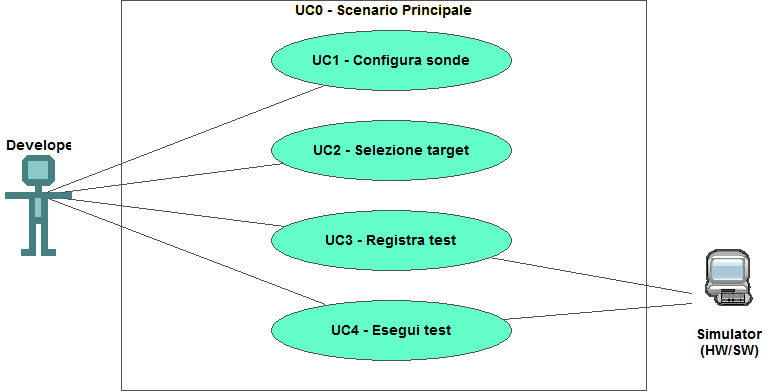
\includegraphics[width=0.9\columnwidth]{usecase/scenario-principale} 
    \caption{Use Case - UC0: Scenario principale}
\end{figure}

\begin{usecase}{0}{Scenario principale}
\usecaseactors{Sviluppatore applicativi}
\usecasepre{Lo sviluppatore è entrato nel plug-in di simulazione all'interno dell'IDE}
\usecasedesc{La finestra di simulazione mette a disposizione i comandi per configurare, registrare o eseguire un test}
\usecasepost{Il sistema è pronto per permettere una nuova interazione}
\label{uc:scenario-principale}
\end{usecase}

\section{Tracciamento dei requisiti}

Da un'attenta analisi dei requisiti e degli use case effettuata sul progetto è stata stilata la tabella che traccia i requisiti in rapporto agli use case.\\
Sono stati individuati diversi tipi di requisiti e si è quindi fatto utilizzo di un codice identificativo per distinguerli.\\
Il codice dei requisiti è così strutturato R(F/Q/V)(N/D/O) dove:
\begin{enumerate}
	\item[R =] requisito
    \item[F =] funzionale
    \item[Q =] qualitativo
    \item[V =] di vincolo
    \item[N =] obbligatorio (necessario)
    \item[D =] desiderabile
    \item[Z =] opzionale
\end{enumerate}
Nelle tabelle \ref{tab:requisiti-funzionali}, \ref{tab:requisiti-qualitativi} e \ref{tab:requisiti-vincolo} sono riassunti i requisiti e il loro tracciamento con gli use case delineati in fase di analisi.

\newpage

\begin{table}%
\caption{Tabella del tracciamento dei requisti funzionali}
\label{tab:requisiti-funzionali}
\begin{tabularx}{\textwidth}{lXl}
\hline\hline
\textbf{Requisito} & \textbf{Descrizione} & \textbf{Use Case}\\
\hline
RFN-1     & L'interfaccia permette di configurare il tipo di sonde del test & UC1 \\
\hline
\end{tabularx}
\end{table}%

\begin{table}%
\caption{Tabella del tracciamento dei requisiti qualitativi}
\label{tab:requisiti-qualitativi}
\begin{tabularx}{\textwidth}{lXl}
\hline\hline
\textbf{Requisito} & \textbf{Descrizione} & \textbf{Use Case}\\
\hline
RQD-1    & Le prestazioni del simulatore hardware deve garantire la giusta esecuzione dei test e non la generazione di falsi negativi & - \\
\hline
\end{tabularx}
\end{table}%

\begin{table}%
\caption{Tabella del tracciamento dei requisiti di vincolo}
\label{tab:requisiti-vincolo}
\begin{tabularx}{\textwidth}{lXl}
\hline\hline
\textbf{Requisito} & \textbf{Descrizione} & \textbf{Use Case}\\
\hline
RVO-1    & La libreria per l'esecuzione dei test automatici deve essere riutilizzabile & - \\
\hline
\end{tabularx}
\end{table}%             % Progettazione e codifica
% !TEX encoding = UTF-8
% !TEX TS-program = pdflatex
% !TEX root = ../tesi.tex

%**************************************************************
\chapter{Confronto tra Angular e React}
\label{cap:angular-react}
%**************************************************************
\intro{In questo capitolo viene effettuato il confronto tra Angular e React. Inizialmente viene presentata una panoramica introduttiva sulle tecnologie in questione, proseguendo poi con un paragone tra i dettagli tecnici e le performance, illustrando infine una riflessione conclusiva. }\\

\section{Introduzione}

\subsection{Angular}
Angular \footcite{site:angular} è una piattaforma \gls{open-sourceg} per lo sviluppo di applicazioni web con \gls{licenza-mit-g}, evoluzione di AngularJS, sviluppata principalmente da Google. \\
\begin{figure}[!h] 
    \centering 
    
\includegraphics[width=0.8\columnwidth]{cap5/angular_logo.png} 
    \caption{Angular Logo}
\end{figure} \\
Angular, essendo un \gls{frameworkg} molto vasto, fornisce diversi strumenti e tecnologie oltre alla possibilità di sviluppo di interfacce utente, tra le quali citiamo la gestione delle rotte, la dependency injection e il two way data-binding. Per questo motivo il \gls{frameworkg} offre agli sviluppatori maggiori soluzioni ai problemi comuni dello sviluppo di applicazioni web rispetto a React, avendo come rovescio della medaglia il fatto di creare dei progetti molto più pesanti a livello di memoria. Quest'ultimo aspetto viene approfondito successivamente nell' \hyperref[sec:performance]{apposita sezione}. \\
Risulta utile citare, infine, che questa tecnologia è arrivata attualmente alla versione 12.1.4 e viene utilizzata da diverse aziende importanti per lo sviluppo del loro software proprietario.  \\
Alcuni esempi di piattaforme create con Angular sono i seguenti: Gmail, MS Office, Paypal, Overleaf.

\subsection{React}
React \footcite{site:react} è una libreria JavaScript \gls{open-sourceg} per la creazione di interfacce utente in applicazioni web, sviluppata e manutenuta principalmente da Facebook. \\
\begin{figure}[!h] 
    \centering 
    
\includegraphics[width=0.7\columnwidth]{cap5/react-logo.jpg} 
    \caption{React Logo}
\end{figure} \\
React, essendo una libreria per la creazione di UI, tende a offrire meno strumenti e soluzioni a problemi comuni dello sviluppo di applicazioni web rispetto ad Angular, dovendosi affidare a librerie esterne create da diverse aziende o dalla community, con il vantaggio di avere un progetto più snello e leggero a livello di memoria. Questo aspetto viene approfondito successivamente nell' \hyperref[sec:performance]{apposita sezione}. \\
Come fatto per la precedente tecnologia, è utile citare il fatto che React sia arrivato attualmente alla versione 17.0.2 e venga utilizzato da diverse aziende importanti per lo sviluppo delle loro piattaforme. \\
Di seguito vengono riportati alcuni esempi di software sviluppato utilizzando React: Airbnb, Discord, Instagram.

\subsection{I componenti}
Tutti i \gls{frameworkg} per il frontend di applicazioni web hanno un obiettivo comune: rendere lo sviluppo web più agevole e trasparente, andando a semplificare molte operazioni che, eseguite con gli strumenti di base come HTML, CSS e Javascript, risultano molto complesse e richiedono molto tempo. \\
La soluzione a questo problema proposta da entrambe le tecnologie in esame, seppur gestita in maniera differente, consiste nei \textbf{component}. \\
Un component corrisponde ad un mattoncino di base per la costruzione di applicazioni web complesse. Ogni component ha il controllo di una determinata sezione di schermo, acquisendone la responsabilità di renderizzare i dati ricevuti e gestire l'interazione con l'utente. Il fatto che ogni component possa averne altri al suo interno crea un modello di programmazione che consente una forte modularità del codice, favorendo il test di unità e la leggibilità del codice stesso.

% ---------------------------------- DETTAGLI TECNICI ----------------------------------------------------

\section{Dettagli tecnici}

\subsection{Linguaggio di programmazione}
\label{sec:linguaggio-programmazione}
\textit{Angular} utilizza come linguaggio di programmazione predefinito \textbf{Typescript}, in quanto la creazione di un progetto avviene attraverso lo strumento dell'Angular CLI \footfullcite{angular-cli} \codeword{ng} e quest'ultimo provvede a creare un workspace che comprende una configurazione di base del linguaggio in questione. \\ \\
\textit{React} invece consiste in una libreria Javascript e, utilizzando lo strumento \codeword{create-react-app} con il package manager npm \footfullcite{npm} per la creazione di un progetto, la configurazione base utilizza proprio il linguaggio \textbf{Javascript}. E' tuttavia possibile configurare un nuovo progetto con il linguaggio Typescript utilizzando lo stesso tool con un ulteriore flag: \codeword{npx create-react-app my-app-name --template typescript}.

\subsection{Gestione dei componenti}
Come è stato descritto nell'introduzione, i component risultano i mattoni di base delle applicazioni web create con entrambe le tecnologie in esame. \\ \\
\textit{Angular} implementa questi componenti utilizzando tre file che consentono di configurare diverse caratteristiche:
\begin{itemize}
	\item \textbf{file.component.ts}: un file Typescript che contiene l'implementazione di una classe nella quale si possono inserire lo stato e le funzionalità offerte all'utente attraverso funzioni che possono agire in modo asincrono ed event-driven;
	\item \textbf{file.component.html}: un file che contiene codice HTML (con la possibilità di estenderne le funzionalità attraverso gli attributi direttive \footfullcite{angular-direttive}) e che corrisponde al template della vista che viene renderizzata dal browser;
	\item \textbf{file.component.css}: un file CSS che contiene lo stile applicabile al template della vista del singolo componente. \\
\end{itemize}
\textit{React} invece implementa questi componenti in un unico file \textbf{component.js} (o component.tsx se il progetto è stato configurato per Typescript) attraverso l'utilizzo del codice \textbf{JSX}, ovvero un'estensione di Javascript (non obbligatoria in quanto è possibile utilizzare anche esclusivamente codice Javascript). \\
Il codice JSX consiste in una sorta di fusione tra un linguaggio di template e il linguaggio Javascript, consentendo di creare "elementi react" che possono essere successivamente renderizzati nel DOM. \\
I component possono essere definiti attraverso l'utilizzo delle classi javascript (implementando un costruttore che consente di settare lo stato e la funzione \codeword{render()}) o attraverso la definizione di una funzione (in questo caso si definisce "componente funzionale).

\subsection{Gestione dello stato}
Lo stato, citato nella sezione precedente, corrisponde a dei dati appartenenti al componente che, se modificati, causano una nuova renderizzazione anche della vista del componente stesso o dei suoi "figli". \\ \\
\textit{Angular} permette la gestione dello stato attraverso il \textbf{two way data-binding}, ovvero la possibilità, attraverso un'apposita sintassi, di legare in due direzioni i dati definiti nella classe (modello) con i dati usati dal template HTML (vista). In questo modo se i dati cambiano nel modello le modifiche vengono riflettute nella vista effettuando un nuovo rendering del componente e, nel verso opposto, se l'utente interagisce con la vista i dati del modello vengono aggiornati automaticamente. \\ \\
\textit{React} invece permette la gestione dello stato solamente attraverso un \textbf{one way data-binding}, ovvero se i dati (modello) vengono modificati allora tale modifica viene riflessa anche nella vista effettuando un nuovo rendering del componente, ma non accade il contrario. Infatti per modificare i dati dello stato è necessario creare apposite funzioni che reagiscano agli eventi innescati dagli elementi presenti nel DOM e che modifichino i dati del modello.

\subsection{Gestione dello stile}
Lo stile da applicare al template HTML è supportato da entrambe le tecnologie, seppur con qualche lieve differenza. \\ \\
\textit{Angular}, come descritto nella sezione relativa ai componenti, utilizza l'apposito \\ \textbf{file.component.css} per applicare lo stile con scope locale (ovvero sul singolo componente) al template HTML definito in un file separato. \\ \\
In \textit{React} invece viene utilizzato principalmente un approccio in cui si usa un \textbf{unico file di stile} con codice CSS con scope globale (ovvero su tutta l'applicazione web). La libreria tuttavia mette a disposizione la possibilità di creare diversi \textbf{moduli CSS} in modo da poter definire gli stessi nomi di classe in file differenti senza il rischio di una collisione tra nomenclature.

% ---------------------------------- PERFORMANCE ----------------------------------------------------

\section{Performance}
\label{subsec:performance}

\subsection{Memoria}
\label{sec:performance}
Come accennato nella \hyperref[sec:introduzione]{sezione introduttiva}, Angular è un \gls{frameworkg} completo, il quale offre molti più strumenti rispetto a React per lo sviluppo di applicazioni web. Questo aspetto, anche se può sembrare un netto punto a favore nei confronti di Angular, va analizzato in modo da valutare pro e contro. \\ \\
\textit{Angular}, attraverso lo strumento apposito della \hyperref[sec:linguaggio-programmazione]{\textsl{Angular CLI}} alla versione 12.1.4, crea un progetto di base dal peso di circa \textbf{344MB} (sul sistema operativo Windows 10 Home). Nel progetto è presente una configurazione di base del linguaggio Typescript, oltre che a strumenti utili come, ad esempio, la gestione delle rotte, il two way data-binding e le librerie jasmine/karma per effettuate unit testing. Tutti questi ottimi strumenti, utili ad uno sviluppatore con l'intento di creare una piattaforma partendo da basi solide, possono tuttavia risultare superflui per creare delle applicazioni web più semplici o a scopo prototipale, rendendo solamente il progetto più pesante a livello di memoria. \\ \\
\textit{React} invece, attraverso l'apposito strumento del \hyperref[sec:linguaggio-programmazione]{\textsl{Node Package Manager}} alla versione 7.19.1, crea un progetto di partenza dalle dimensioni su disco di circa \textbf{215MB} (sul sistema operativo Windows 10 Home). Come si può notare il workspace creato da React risulta molto più leggero in memoria, avvicinandosi alla metà delle dimensioni rispetto a quello generato con Angular, offrendo certamente meno servizi allo sviluppatore. Infatti risultano disponibili, oltre alla libreria jest per effettuare unit testing, pochi altri servizi necessari al funzionamento dell'applicazione web. Questo aspetto consente, specialmente ad uno sviluppatore esperto, di integrare attraverso il proprio package manager solamente le funzionalità di cui si ha bisogno in modo modulare, anche se ciò potrebbe risultare problematico ai programmatori novizi.

\subsection{Site Rendering}
\label{sec:site-rendering}
Entrambe le tecnologie, per fornire al browser il documento da visualizzare a schermo, utilizzano di base il \textbf{Client-Side Rendering (CSR)}. Con una soluzione di rendering lato client, il server esegue il rendering di una pagina vuota con un dei riferimenti ai file Javascript dell'applicazione web. La pagina vuota viene inviata al browser client, che inizia a eseguire l'app, compila il tutto, quindi effettua le chiamate \gls{api} necessarie e a visualizzare il contenuto della pagina. \\
Questa modalità di rendering consente di dare poco carico di lavoro al server in quanto invia una pagina vuota al client, tuttavia presenta problemi di diverse tipologie, ad esempio nel caso in cui l'applicazione web è di grandi dimensioni e il client ha una connessione lenta, poiché subirà un notevole ritardo nel caricamento e vedrà la pagina renderizzata solo quando sarà presente tutto il contenuto (causando un lungo caricamento con una pagina vuota alla prima navigazione). \\
Per ovviare a questo problema sono disponibili principalmente due tecniche di pre-rendering:
\begin{itemize}
	\item \textbf{Server-Side Rendering (SSR)}: corrisponde alla capacità di un'applicazione di contribuire alla visualizzazione della pagina web sul server invece di renderizzarla nel browser. Ciò significa che se di un'applicazione viene eseguito il rendering lato server, il suo contenuto corrisponde a codice HTML che viene generato in anticipo dal server e successivamente passato al browser del client per essere visualizzato dall'utente. Con il rendering lato client è diverso, in quanto bisogna navigare su una pagina prima che vengano recuperati i dati dal server, il che significa che l'utente dovrebbe aspettare alcuni secondi prima di ricevere il contenuto della pagina per poterla finalmente renderizzare. Questa modalità di rendering effettua il fetch delle risorse necessarie per creare il contenuto della pagina web ad ogni richiesta da parte del client e ha alcuni vantaggi, tra i quali la possibilità di visualizzare quasi istantaneamente le pagine web (al costo di un maggior carico di lavoro al server) e un miglioramento delle performance SEO.
	\item \textbf{Static-Site Generation (SSG)}: consiste in un'applicazione software che crea pagine HTML da modelli o componenti e da una determinata fonte di contenuto. La generazione statica del sito è simile al server-side rendering con l'eccezione che si esegue il rendering delle pagine in fase di build anziché ad ogni richiesta da parte del client. Questo significa che le pagine dell'applicazione web vengono generate al momento della build e il contenuto del sito non cambia a meno che non vengano aggiunti nuovi contenuti o component e venga effettuato nuovamente la build. Un'ulteriore possibilità (implementabile ad esempio nel \gls{frameworkg} Next.js), consiste nell'effettuare una nuova build del sito dopo un determinato e regolare intervallo di tempo, in modo da dare la possibilità al server di capire se sono presenti modifiche nelle risorse utilizzate per il contenuto delle pagine web. \\
\end{itemize}
\textit{React} di base fornisce esclusivamente il Client-Side Redering, tuttavia è una libreria integrata dal \gls{frameworkg} \textbf{Next.js} \footfullcite{nextjs}, il quale offre sia Server-Side Rendering che Static-Site Generation e una soluzione ibrida tra queste, come citato precedentemente.
\begin{figure}[H] 
    \centering 
    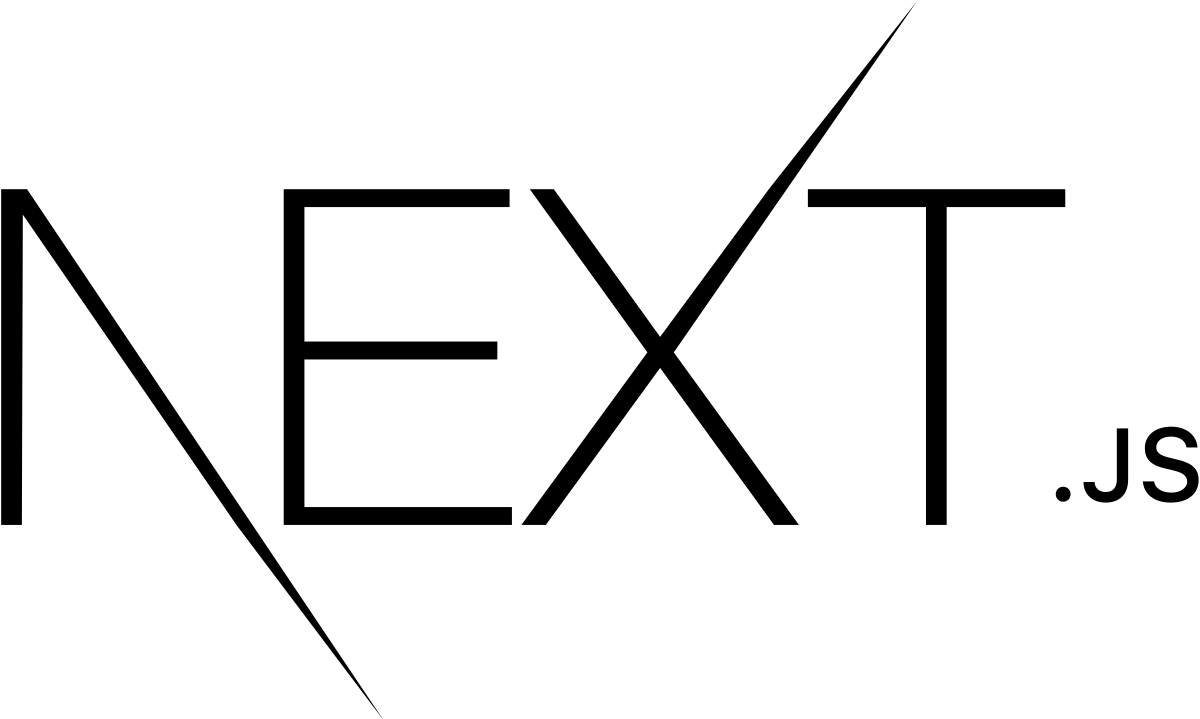
\includegraphics[width=0.35\columnwidth]{cap5/nextjs-logo} 
    \caption{Next.js Logo}
\end{figure}
\noindent Anche \textit{Angular} fornisce di base esclusivamente il Client-Side Rendering, tuttavia è possibile integrare le tecnologie \textbf{Angular Universal} \footfullcite{angular-universal} per permettere il Server-Side Rendering e \textbf{Scully} \footfullcite{scully} per offrire lo Static-Site Generation.
\begin{figure}[!h] 
    \centering 
    
\includegraphics[width=0.45\columnwidth]{cap5/angular-universal-logo} 
    \caption{Angular Universal Logo}
\end{figure}

\subsection{Rendering della UI}
Parlando di performance di applicazioni web la dimensione non risulta un problema particolare, soprattutto quando si tratta di software di grandi dimensioni. Ciò che influisce maggiormente sulle prestazioni di runtime è la modalità di manipolazione del Document Object Model (DOM), ovvero la rappresentazione dell'ipertesto strutturata come modello orientato agli oggetti. Infatti la manipolazione del DOM risulta il cuore del web moderno e interattivo anche se, sfortunatamente, è anche molto più lento della maggior parte delle operazioni JavaScript. Per questo motivo è fondamentale analizzare come le due tecnologie implementano l'interazione con il DOM per valutarne le performance. \\ \\
\textit{Angular} utilizza e manipola direttamente il \textbf{DOM reale} e sfrutta il data-binding bidirezionale, quindi tutte le modifiche apportate al modello vengono replicate anche nella vista. Durante la traduzione di un'applicazione pesante, potrebbero quindi rallentare le prestazioni. \\ \\
\textit{React} invece utilizza il \textbf{Virtual DOM}, ovvero una copia più leggera del DOM realmente utilizzato per rendere dinamica l'applicazione. Per ogni oggetto DOM c'è un corrispondente oggetto DOM virtuale che corrisponde a una sua rappresentazione con le stesse proprietà, ma senza il potere di cambiare direttamente ciò che è presente a schermo. Mentre la manipolazione del DOM è lenta, quella del DOM virtuale è molto più veloce perché nulla viene renderizzato sullo schermo. \\
L'utilità del DOM virtuale consiste nel fatto che quando viene eseguito il rendering di un elemento JSX, ogni singolo oggetto DOM virtuale viene aggiornato molto rapidamente.
Una volta che il DOM virtuale è stato aggiornato, React confronta il DOM virtuale con un'istantanea dello stesso che è stata scattata subito prima dell'aggiornamento. Effettuando questa operazione React scopre esattamente quali oggetti DOM virtuali sono cambiati (processo di Diffing). Questo permette a React di aggiornare solamente gli oggetti necessari nel DOM reale, senza effettuare inutili rendering di oggetti che sono rimasti inalterati. \\
Grazie a questa tipologia di innovazione nell'interazione con il DOM React può vantare di avere delle prestazioni nel rendering della user interface migliori rispetto ad Angular.

% ---------------------------------- CONCLUSIONI ----------------------------------------------------

\section{Conclusioni}

\textit{Angular}:
\begin{itemize}
	\item consiste in un \gls{frameworkg} ricco e completo, molto basato su Typescript;
	\item è un \gls{frameworkg} opinionated, ovvero limita o guida in modo molto stringente nel modo di fare le cose, risultando uno svantaggio per gli sviluppatori che vogliono costruire soluzioni diverse da quelle standard ma un vantaggio in quanto limita molto la probabilità di errori nel codice;
	\item possiede un'ottima documentazione dei suoi strumenti;
	\item richiede un certo tempo per essere appreso in modo efficacie in quanto è necessario studiare un intero ecosistema;
	\item consente di dare una struttura solida al progetto sin dalla sua creazione e risulta adatto per applicazioni di grandi dimensioni senza un eccessivo quantitativo di aggiornamenti a schermo. \\
\end{itemize}
\textit{React}:
\begin{itemize}
	\item consiste in una libreria per sviluppo di interfacce grafiche, molto basata su Javascript, quindi molto leggera ma dipendente da librerie terze per effettuare molte operazioni necessarie allo sviluppo web;
	\item è unopinionated, quindi risulta molto flessibile e potente per sviluppatori esperti ma con probabilità più alta di commettere errori nel codice rispetto ad Angular;
	\item può vantare una community più vasta ed attiva rispetto ad Angular;
	\item richiede un tempo di apprendimento minore rispetto ad Angular rendendo disponibili meno strumenti da imparare;
	\item consente di effettuare progetti in modo più libero e veloce, risultando particolarmente utile quindi per creare prototipi e molto appetibile per utenti principianti che possiedono una base di Javascript. \\ \\
\end{itemize}
In conclusione all'analisi effettuata in questo documento è possibile affermare che nel dibattito Angular vs React non c'è una scelta migliore. Ogni soluzione ha i suoi vantaggi e svantaggi, si adatta a diverse tipologie di progetto e gruppi di lavoro. \\
Personalmente durante lo sviluppo del progetto Voting-Online ho preferito usare Angular in quanto, una volta superata la fase iniziale di apprendimento, mi ha fornito tutti gli strumenti di cui avevo bisogno per creare l'applicazione web, mentre per effettuare le stesse operazioni con React mi sono trovato più volte a dover installare diverse librerie scritte da utenti della community che risultavano a volte limitate o comunque scarsamente documentate.             % Confronto Angular React
% !TEX encoding = UTF-8
% !TEX TS-program = pdflatex
% !TEX root = ../tesi.tex

%**************************************************************
\chapter{Verifica e validazione}
\label{cap:verifica-validazione}
%**************************************************************             % Conclusioni
%\appendix                               
%% !TEX encoding = UTF-8
% !TEX TS-program = pdflatex
% !TEX root = ../tesi.tex

%**************************************************************
\chapter{Appendice A}
%**************************************************************

\epigraph{Citazione}{Autore della citazione}



             % Appendice A

%**************************************************************
% Materiale finale
%**************************************************************
\backmatter
\printglossaries
% !TEX encoding = UTF-8
% !TEX TS-program = pdflatex
% !TEX root = ../tesi.tex

%**************************************************************
% Bibliografia
%**************************************************************

\cleardoublepage
\chapter{Bibliografia}

\nocite{*}
% Stampa i riferimenti bibliografici
\printbibliography[heading=subbibliography,title={Riferimenti bibliografici},type=book]

% Stampa i siti web consultati
\printbibliography[heading=subbibliography,title={Siti web consultati},type=online]


\end{document}
